% !TeX program = xelatex
% Korean counterpart of SweepBasedCollisionAvoidanceFramework_en.tex.
% Section order, equations, figures, data, and bibliography follow the English version.
\documentclass[11pt,a4paper]{article}
\usepackage[margin=25mm]{geometry}
\usepackage[no-math]{fontspec}
\setmainfont{Malgun Gothic}[ItalicFont={Malgun Gothic},ItalicFeatures={FakeSlant=0.15}]
\newfontfamily\latinfont{Times New Roman}
\setsansfont{Malgun Gothic}
\setmonofont{Consolas}
\XeTeXlinebreaklocale "ko"
\XeTeXlinebreakskip=0pt plus 0.5pt
\usepackage{amsmath,amssymb,amsthm,booktabs}
\usepackage{tikz,graphicx,longtable}
\graphicspath{{Figures/}{docs/RMFS/Papers/2026_11_SweepBasedCollisionAvoidanceFramework/Figures/}}
\usetikzlibrary{arrows.meta,positioning}
\usepackage[hidelinks]{hyperref}
\newtheorem{definition}{정의}
\newtheorem{proposition}{명제}
\newtheorem{theorem}{정리}
\theoremstyle{remark}
\newtheorem{remark}{주석}
\renewcommand{\proofname}{증명}
\renewcommand{\abstractname}{초록}
\renewcommand{\figurename}{그림}
\renewcommand{\tablename}{표}
\renewcommand{\refname}{참고문헌}
\newcommand{\Sw}{\mathcal S}
\newcommand{\Rs}{\mathcal R}
\newcounter{algorithm}
\newcounter{algline}
\providecommand{\theHalgline}{\arabic{algorithm}.\arabic{algline}}
\newcommand{\algl}[3]{\refstepcounter{algline}\label{#1}\item[\arabic{algline}.]\hspace*{#2em}#3}
\newenvironment{pseudocode}[2]{%
  \par\medskip\noindent\begin{minipage}{\linewidth}\refstepcounter{algorithm}\label{#1}
  \noindent\textbf{알고리즘 \thealgorithm. #2}\par\smallskip
  \hrule\smallskip\begingroup\small\setcounter{algline}{0}
  \begin{list}{}{\setlength{\leftmargin}{2em}\setlength{\labelwidth}{1.5em}\setlength{\labelsep}{.5em}\setlength{\itemsep}{3pt}}
}{\end{list}\endgroup\smallskip\hrule\end{minipage}\par\medskip}
\title{이동 로봇의 충돌 회피를 위한\\스윕 기반 프레임워크}
\author{Moon Ho Hwang\\\small\href{mailto:moon.hwang@gmail.com}{\texttt{moon.hwang@gmail.com}}}
\date{2026년 11월 22일\\\small 연구 원고 · 이론, 구현 및 예제}
\begin{document}
\maketitle
\begin{abstract}
본 논문은 여러 이동 로봇이 주어진 경로를 충돌 없이 유한시간에 완료하도록 기존 스윕 기반 조정 원리를 정식화하고 구현한다. 물리적 시간을 추상화하면서 이동 순서를 유지한다. 점유영역 스윕의 교차로 간섭을 표현하고, 양립 가능한 이동과 대기를 완전한 묶음경로로 구성한다. 점분스 복사는 대기를 표현하며, 안전한 분스합은 원래 제어 제약을 유지하면서 연속 이동을 결합한다. 완료 충분조건을 도출하고, 필요한 간섭 순서를 유지하는 구성 및 실행 알고리즘을 제시한다. 명시된 기하학적·실행 가정 아래 무충돌 실행과 유한시간 완료가 성립한다. 정식화는 일반 점유영역을 다루며, 구현과 실험은 2차원 직사각형 충돌 외곽을 사용하는 이동 로봇에 적용한다.

FIFO와 최장 잔여 경로(LP)는 안전 및 완료 조건을 만족하는 동작 중에서 선택한다. DEVS 시뮬레이션~\cite{zeigler1976,zeigler2018}으로 수정 후 정차 방식의 기준 성능을 검증했다. 세 로봇의 관찰 예제부터 방향성 간섭 구간 631개와 총간섭 길이 2,581~m를 갖는 50대의 내부 교통까지, 고정 경로 집합 13개를 평가했다. 26개 정책 조건 모두 시간 측정 실행을 세 번씩 완료했으며, 독립 충돌 정지 재실행에서도 충돌이나 교착이 검출되지 않았다. 이 결과는 구현이 검증 사례에서 유도한 안전 및 완료 성질을 만족함을 보여준다. 간섭과 완료 조건은 향후 새 목적지에 대한 간섭 고려 경로 생성 연구의 바탕이 된다.
\end{abstract}
\noindent\textbf{핵심어} 스윕 볼륨, 충돌 회피, 이동 로봇, 다중 로봇 경로계획, 로봇 이동형 주문 처리 시스템(RMFS), DEVS.

\section{서론}
두 이동체의 경로 스윕이 겹쳐도 공유 공간을 서로 다른 시각에 점유하면 충돌하지 않는다. 반대로 다른 이동체가 대기할 때 안전한 이동도 이후의 완료를 막을 수 있다. 따라서 스윕의 겹침과 다음 순간의 배치에 더해 전체 이동 순서를 검토해야 한다.

본 연구는 주어진 순서 경로를 이동과 대기로 실행하는 문제를 다룬다. 경로 생성과 운송 주문 배정은 실험 범위 밖이다. 목표는 충돌 없이 전체 경로를 완료하는 실행을 구성하는 것이다.

\paragraph{프레임워크와 구현의 범위}
경로, 점유영역, 스윕 및 묶음 정의는 명시한 기하 및 실행 가정을 만족하는 일반 형상에 적용된다. 구현은 2차원 축 정렬 직사각형 점유 외곽과 축 정렬 경로를 사용한다. 이로써 스윕의 구성과 교차 판정을 명시적으로 구현할 수 있다. 일반 형상의 연산 비용은 기하에 따라 달라진다.

\begin{enumerate}
\item 경로와 부분경로 스윕, 완전한 $n$개 물체의 묶음경로를 정의한다.
\item 순차 충분조건이나 유한 점분스 복사 탐색으로 묶음경로를 구성하고 검증한다.
\item 허가, 피드백, 해제와 명령 병합 알고리즘으로 묶음경로를 실행한다.
\item 실행 보장의 가정을 명시하고 Plant 실행과 유한 분류를 검증한다.
\end{enumerate}
\ref{sec:construction}--\ref{sec:control-guarantees}절은 실행 가능한 묶음의 존재, 구성 절차, 실행 규칙 및 보장을 구분한다. 단순 경로와 복잡한 고정 경로 사례에 동일한 안전 및 완료 조건을 적용해 두 교통 정책을 평가한다. 잔여 간섭 그룹은 분해와 모니터링을 지원한다. 작업 기반 확장의 증명 개요는 보고된 해제와 출발 조건이 간섭 순서 및 전체 진행을 보존하는 과정을 설명한다.

\section{선행연구와의 관계}
\label{sec:prior-art}
\subsection{직접 선행연구: 1989년의 구간 스윕 조정}
O'Donnell과 Lozano-P\'erez~\cite{odonnell1989}는 두 매니퓰레이터의 지정 경로를 순서가 있는 구간의 스윕으로 표현해 무충돌 일정을 구성했다. 작업 완료 도표의 셀은 물리 공간의 격자가 아니라 구간 쌍이다. 수평·수직·대각선 진행은 각각 한 로봇의 이동, 다른 로봇의 이동, 동시 이동을 뜻한다. START/WAIT 실행에서는 구간 완료가 후속 동작을 허용한다. 논문 486쪽은 길이가 0인 끝점 구간과 종점 정차로 인한 차단을 다루고, 487쪽은 전체 경로의 순차 실행이 불가능할 때 전역 일정을 탐색한다.
\begin{table}[htbp]
\centering\small
\caption{1989년 구간 스윕 구성과의 대응. 각 행은 동일한 조정 원리의 표현을 대조한다.}
\label{tab:1989-correspondence}
\begin{tabular}{p{.29\linewidth}p{.62\linewidth}}
\toprule
본 논문의 용어 & 해당 선행 개념~\cite{odonnell1989}\\\midrule
부분경로 스윕 & 순서가 있는 구간의 스윕 볼륨.\\[3pt]
점분스 및 종점 점유 & 길이 0인 끝점 구간과 유지되는 점유로 인한 차단.\\[3pt]
양립 가능한 스윕 쌍 & 작업 완료 도표의 양립 가능한 구간 쌍.\\[3pt]
점 대기 복사 & 한 진행 좌표를 유지하면서 상대가 진행.\\[3pt]
교대 부분 진행 & 수평 및 수직 일정 진행을 교대로 적용.\\[3pt]
시각을 지정하지 않은 순서 & 구간 완료로 발행하는 START/WAIT 명령.\\
\bottomrule
\end{tabular}
\end{table}

\paragraph{유한 모델의 대응}
두 경로의 엣지 수 $m_i,m_j$, 정점 정차점, 점유 외곽 및 보수적인 스윕 판정을 고정한다.
\begin{equation}
\begin{split}
 Q_{ij}&=\{0,\ldots,m_i\}\times\{0,\ldots,m_j\},\\
 (k,l)&\longrightarrow(k+d_i,l+d_j)
 \quad\Longleftrightarrow\quad
 \Sw_i[k,k+d_i]\cap\Sw_j[l,l+d_j]=\varnothing.
\end{split}
\label{eq:prior-progress}
\end{equation}
$(d_i,d_j)\in\{(1,0),(0,1),(1,1)\}$이고 후속 상태는 $Q_{ij}$ 안에 있어야 한다. $\Sw_i[k,k]$는 정점 $k$에서의 대기 점유다. 이 비교에서는 스윕 인수가 엣지 진행을 나타낸다. 초기 점유는 서로 겹치지 않고 종점 점유는 유지된다.

본 연구의 전수 점분스 복사 모델과 고전 구간 진행 그래프는 이 유한 입력에서 동일한 완료 도달성을 갖는다. 점 토큰만 소비하는 단계를 지우면 나머지는 허용된 진행이 된다. 반대로 각 진행 전후에 다른 로봇을 대기시키며 안전한 원래 정점 토큰을 삽입할 수 있다. 토큰 점유는 안전한 진행 스윕의 부분집합이므로 두 변환 모두 안전과 경로 순서를 보존한다. 이 대응은 해당 유한 모델에 관한 것이다. 16개 끝점 분류 역시 제한된 특성화다. 검토한 문헌에서 동일한 4비트 표를 찾지 못했다는 사실만으로 신규성을 확립할 수는 없다.

\subsection{후속 조정 연구와 피드백 실행}
Leroy 등~\cite{leroy1999}은 기하학적 조정 도표와 상호작용 분해를 사용하며 후진도 허용한다. Gr\'egoire 등~\cite{gregoire2015}의 3.2절 정리 3은 비순환 우선관계를 위상 정렬해 로봇을 순차 완료시키는 구성이다. 본 연구의 충분조건도 같은 구성 방식을 사용하며 기하와 끝점 가정은 서로 다르다. RMTRACK~\cite{cap2016}은 지연 외란에서 기존 통과 순서를 보존한다. ADG~\cite{hoenig2019}는 완료 보고를 사용하고 피드백을 유지하면서 전진 명령을 병합한다. Segment Graph~\cite{coskun2021}는 간섭 경계에서 경로를 나누고 순서 변경에 따른 교착을 검사하며, 타 로봇의 시작점과 종점을 피하는 궤적을 가정한다. SADG~\cite{berndt2024}는 MILP로 허용 의존성을 재정렬하고 명시된 가정 아래 재귀적 실행 가능성을 보인다. 유효한 초기 계획 구성과 그 실행은 별도 과제다.

\subsection{시간 기반 통과 순서 수정}
\label{sec:time-repair-review}
Coskun과 O'Kane~\cite{coskun2019}의 V절은 선행권 때문에 대기하지만 상대가 도착하기 전에 공유 공간을 비울 수 있는 사례를 다룬다. 로봇마다 장애물에 처음 차단될 때 한 번만 순서 반전을 검사한다. TestFlipFast는 조정 장애물의 경계 상자로 예상 해제와 진입 시각을 비교한다. TestFlipAggressive는 공동 진행을 모델링해 기존 순서와 반전 순서에서 두 로봇의 예상 해제 시각 합을 비교한다. 외란 추정에는 가우시안 과정 회귀를 사용한다. 검사가 성공하면 우선권 표지를 변경하며, 실제 운동은 RMTRACK이 계속 제어한다. 예상 시간 비교는 국소 성능 판단이며 예측 구간 내 공간 해제를 보증하지 않는다.
\begin{figure}[htbp]
\centering
\begin{tikzpicture}[x=.85cm,y=.8cm,>=Stealth,every node/.style={font=\small}]
\draw[->] (0,0)--(11,0) node[right] {$t$};
\foreach \x in {0,1,4,8,10} {\draw (\x,.07)--(\x,-.07) node[below] {\x};}
\filldraw[fill=red!20,draw=red!65!black] (1,.6) rectangle (4,1.2);
\node at (2.5,.9) {$i$: 점유};
\filldraw[fill=blue!15,draw=blue!65!black] (8,1.6) rectangle (10,2.2);
\node at (9,1.9) {$j$: 점유};
\draw[<->] (4,.35)--node[above,font=\footnotesize]{시간 간격}(8,.35);
\node[anchor=west] at (0,2.75) {같은 공간에서 겹치지 않는 점유 시간 구간};
\end{tikzpicture}
\caption{공유 공간의 점유 시각을 설명하는 예시. 스윕이 겹쳐도 점유 시각이 분리될 수 있다. 예상 시간 차이는 강제 가능한 순서 및 오차가 제한된 시각과 구분한다.}
\label{fig:timed-separation}
\end{figure}

Segment Graph~\cite{coskun2021}의 정의 2--4와 알고리즘은 간섭 경계에서 나눈 부분경로를 정점으로 사용한다. 엣지는 자체 경로 순서 및 로봇 간 완료 후 출발 조건을 보존한다. 순서 반전은 선행 엣지를 바꾸고 순환 검사는 순환 대기를 유발하는 변경을 배제한다. 비순환에서 교착 부재를 도출하려면 상대의 초기 및 최종 자세를 피해야 한다. 해당 논문의 그림 4에는 순환이 없는 끝점 차단도 있다. 이산 단계와 원형 로봇 모델의 보장을 임의 주문 경로나 연속 가속도 모델에 바로 적용할 수는 없다.

\paragraph{검토할 적용 방법}
공유 공간 $C$의 예상 상대 시각과 보증된 시간 경계를 구분한다. 빠른 성능 검사는 다음과 같다.
\begin{equation}
 \widehat{\tau}^{\rm clear}_{i,C}
 < \widehat{\tau}^{\rm enter}_{j,C}.
 \label{eq:estimated-gap}
\end{equation}
더 강한 충분조건에는 다음과 같이 진입 가능한 모든 상대 로봇에 대한 경계가 필요하다.
\begin{equation}
 \overline{\tau}^{\rm clear}_{i,C}+\eta
 <\min_{j\ne i}\underline{\tau}^{\rm enter}_{j,C},
 \label{eq:bounded-gap}
\end{equation}
상한은 몸체 전체의 최후 해제 시각을, 하한은 상대의 최초 진입 시각을 포함한다. $\eta$는 음이 아닌 여유 시간이다. 이 조건은 본 연구의 공학적 제안이다. 임의로 긴 지연이 가능하면 유한 해제 상한을 보장하기 어렵다. 다른 방법은 상대 로봇이 안전하게 멈출 수 있는 위치에서 실제 해제까지 대기하는 것이다.

국소 간섭 구간을 찾고, 순서 변경의 이득을 추정한 뒤 선행관계·종점 점유·정차 조건을 검사한다. 변경 예약은 일관되게 기록하고 실제 해제를 보고받아 실행한다. 발행한 명령은 암묵적으로 취소할 수 없다. 하류 차단은 해제 추정에 포함하거나 예약으로 배제해야 한다. 현재 TrafficManager의 시간 기반 순서 수정은 후속 과제로 남아 있다.

\subsection{감속 전 통과 결정}
\label{sec:prebraking-review}
후속 연구는 다음 정차점을 향한 감속에 들어가기 전에 간섭영역을 계속 통과할 수 있는지를 판단한다. 결정론적 가상 트윈에서는 주행 중인 상태를 분기점으로 삼는다.

\paragraph{감속 경계 이벤트의 선행연구}
Quesel 등~\cite{quesel2016}의 5.3절 예제 3a는 정지 표지 제어의 최종 제동 경계를 다음과 같이 정의한다.
\begin{equation}
 p+\frac{v^2}{2B}=S,
 \label{eq:braking-boundary}
\end{equation}
$p$는 차선상의 위치, $v$는 속도, $B>0$은 감속의 크기, $S$는 정차 위치다. 제어기가 실행될 수 있는 최후 경계이며 그보다 먼저 실행할 수도 있다. 5.5절은 이상적 이벤트 검출과 표본 센싱을 구분한다. 가상 트윈에서는 이를 해석적으로 예약할 수 있다. 최종 제동 경계는 선택한 승차감 중심 프로파일의 감속 개시점보다 늦을 수 있다.

\paragraph{진입 전 시뮬레이션 허가}
Dresner와 Stone~\cite{dresner2008}의 3.3--3.4절 및 부록 C에서는 접근 차량이 도착 시각과 속도를 요청한다. 교차로 관리자는 기존 시공간 타일 예약과 통과 동작을 시뮬레이션한다. 승인하면 예약하고 거절하면 차량이 감속하면서 재요청한다. 진입 전 시뮬레이션과 무정차 통과, 가속 대안이 이미 포함된다. 식~\eqref{eq:braking-boundary}과 일치하는 의무적 호출 시점은 검토한 절에 없으며, 전체 DEVS 차량군 복제와 후보 차량의 예약 검사는 범위가 다르다.

\paragraph{제동선 기반 정차 또는 통과}
Kalose 등~\cite{kalose2024}의 5.1--5.2절 및 그림 5는 속도와 감속 단계로 제동선을 계산한다. 제동선에 대한 상대 위치와 신호 상태에 따라 통과 또는 단계 감속을 선택하며, 녹색 신호는 교차로 접근 감속 없이 통과를 허용한다.
\begin{table}[htbp]
\centering\small
\caption{감속 전 lookahead 제안의 각 구성 요소에 직접 대응하는 선행 근거.}
\label{tab:prebraking-review}
\begin{tabular}{p{.24\linewidth}p{.33\linewidth}p{.34\linewidth}}
\toprule
문헌 & 직접 관련된 결과 & 제안과의 차이\\\midrule
Quesel 등~\cite{quesel2016} & 최종 제동 경계 이전 또는 경계에서 제어 호출. & 정지 표지 안전 제어.\\[4pt]
Dresner--Stone~\cite{dresner2008} & 진입 전 통과 시뮬레이션 및 예약. 거부 시 감속. & 기존 예약에 대한 후보 통과 검사. 의무적 제동 경계 호출은 확인되지 않음.\\[4pt]
Kalose 등~\cite{kalose2024} & 속도와 제동선에 따른 정차 또는 통과. & 신호 상태를 사용하는 국소 제어.\\[4pt]
DEVS 후속 연구 제안 & 예정 감속 전 이벤트에서 이동 상태를 분기하고 다음 영역의 해제를 검사. & 구현, 검증 및 신규성 확인이 필요한 제안.\\
\bottomrule
\end{tabular}
\end{table}

\paragraph{검증할 실험}
등감속에서 안전 정차점까지의 전방 거리 $d_i(t)$에 대해 $d_i(t_b)=v_i(t_b)^2/(2b_i)$, $v_i(t_b)>0$, $b_i>0$인 이벤트를 계산한다. 여유 거리를 추가한 조기 요청이나 일반 프로파일의 정차거리 함수도 적용할 수 있다. $t_b$에서 위치·속도 및 제어 상태를 저장하고, 통과 대안을 몸체 전체의 다음 간섭영역 해제까지 모의 실행한다. 안전하게 비울 수 없으면 정차 대안을 따른다. 채택한 분기의 명령과 예약은 부모 실행에 반영한다. 이 검사는 국소 통과 가능성을 다루며 전체 완료 가능성은 별도로 유지해야 한다. 회전에 물리적으로 필요한 정차는 유지된다.

세 가지 비교 요소는 \textbf{결정 시점}(정차 후 또는 선택 프로파일의 감속 시작), \textbf{평가 상태}(위치·속도·진행 중 운동·예정 이벤트·예약·제어기를 담은 차량군 스냅샷 또는 기존 예약표), \textbf{국소 종료 조건}(다음 간섭영역의 완전 해제)이다. 동일 경로, 외곽 및 운동 한계에서 결정 시각의 효과와 평가법의 효과를 분리한다. 원 구현을 재현하지 않은 비교 구현은 문헌 방법의 적용판으로 명시한다. 허가 판단의 불일치, 피한 정차, 대기시간, 전체 완료시간, 호출 수와 실제 계산시간을 보고한다. 두 평가법이 항상 같은 결정을 내리면 구현 방식이나 계산 비용의 차이를 보여준다. 이 비교는 후속 연구이며, 관련 요소들은 앞선 연구에서 각각 확인된다.

\subsection{SCALE과 포함 관계}
SCALE~\cite{scale2026}은 로드맵 계획과 국소 수정, 이종 기하 충돌 판정, 동작 선행 그래프(HAPG), 동작 캡슐 및 제한 지평 MILP 순서 변경을 결합한다. 점유 스윕은 병진과 회전을 포함한다. 유한 비트 점유 표현 자체는 물리 공간의 정규 격자를 뜻하지 않는다.

같은 정사각형 외곽과 실행 가능한 동작 순위를 사용하면 본 연구의 교대 진행 예제를 HAPG로 표현할 수 있다. 로봇 간 엣지는 4개이며 추이 축약 후 대응 ADG와 같은 의존성 2개가 남는다. 로봇 수준의 순환은 동작별 의존성을 유지하면 사라진다. 이는 분석적 변환이다. SCALE의 경로 생성·수정과 순서 최적화는 본 연구의 고정 경로 실행보다 넓다. 제시된 MILP는 예측 지평 이탈 시각의 합을 최소화한다.
\begin{figure}[htbp]
\centering
\resizebox{\linewidth}{!}{%
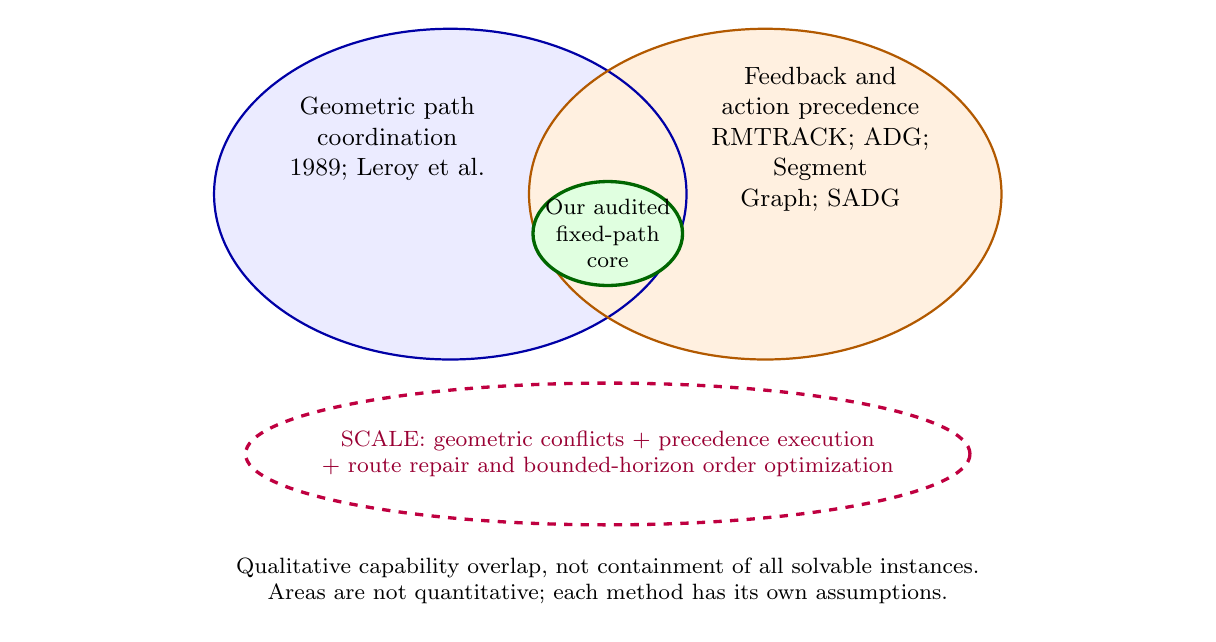
\begin{tikzpicture}[every node/.style={font=\small,align=center}]
\fill[blue!8] (3,2) ellipse (3 and 2.1);
\fill[orange!12] (7,2) ellipse (3 and 2.1);
\draw[thick,blue!65!black] (3,2) ellipse (3 and 2.1);
\draw[thick,orange!70!black] (7,2) ellipse (3 and 2.1);
\node[text width=30mm] at (2.2,2.7) {Geometric path\\coordination\\1989; Leroy et al.};
\node[text width=32mm] at (7.7,2.7) {Feedback and\\action precedence\\RMTRACK; ADG;\\Segment Graph; SADG};
\draw[very thick,green!40!black,fill=green!12] (5,1.5) ellipse (.95 and .66);
\node[text width=18mm,font=\footnotesize] at (5,1.5) {Our audited\\fixed-path\\core};
\draw[very thick,dashed,purple] (5,-1.3) ellipse (4.6 and .9);
\node[text width=80mm,font=\footnotesize,purple!80!black] at (5,-1.3) {SCALE: geometric conflicts + precedence execution\\+ route repair and bounded-horizon order optimization};
\node[anchor=north,text width=145mm,font=\footnotesize] at (5,-2.5)
{Qualitative capability overlap, not containment of all solvable instances.\\
Areas are not quantitative; each method has its own assumptions.};
\end{tikzpicture}}
\caption{기존 연구와 본 구현의 개념적 기능 중첩. 초록색은 구현이 사용하는 기존 원리를 표시한다. 영역의 크기는 정량 의미가 없으며, 해결 가능한 사례의 포함 정리를 나타내지 않는다.}
\label{fig:prior-art-overlap}
\end{figure}

식~\eqref{eq:prior-progress}은 고정된 두 로봇의 유한 추상화에 대한 도달성 대응을 설명한다. 모든 해결 사례에 대해 $\mathcal F_{\rm ours}\subseteq\mathcal F_{\rm SCALE}$를 주장하려면 외곽, 정차, 끝점 점유, 허용 운동, 탐색 범위, 지평과 시간 제한을 일치시켜야 한다. 끝점 표, 점 토큰 관리, 직사각형 RMFS 구현 및 시간을 포함한 DEVS Plant가 확인된 구현 특성이다. 독립적인 이론 우위나 계산 성능 우위는 별도 검증 대상이다.

\subsection{기하 모델과 구현 근거}
H\"onig 등~\cite{hoenig2019}의 III--IV절은 4연결 격자의 정점·엣지 충돌과 연속시간 실행을 위한 동작 의존성 그래프를 사용한다. 물리 안전성은 셀 크기, 로봇 직경, 허용 동작과 연결된다. 다른 통로 그래프에서는 엣지가 달라도 실제 스윕이 겹치거나, 반대로 큰 예약 셀이 서로 만나지 않는 이동을 배제할 수 있다. 점유 외곽과 추가 충돌 규칙이 이러한 차이를 다룬다. MiR600 제조사 자료~\cite{mir600guide}의 지도 기반 전역 계획과 국소 장애물 회피는 논리적 교통 자원과 실제 이동 기하를 구분할 이유를 보여준다.

Leroy 등~\cite{leroy1999}은 정규 공간 격자 없이 최대 150대 사례를 보고했다. 상호작용 그룹 분해가 효율을 좌우하며, 큰 연결 그룹에서는 탐색 차원이 증가한다. 해당 구현이 제시한 실용 그룹 크기는 약 10대다. \AA blad 등~\cite{ablad2021}은 적응적 여유 샘플링으로 거리 질의 비용을 줄이고 명시적 옥트리 교차와 비교했다. 기하 질의와 조합 조정은 별개의 확장 비용이다. 고정 경로 스윕 조정에는 이미 여러 이론적 토대가 있다~\cite{odonnell1989,leroy1999,gregoire2015,cap2016}.

본 연구의 구현은 묶음 구성, 순서 보존 실행, 보고 기반 잔여 해제를 연결한다. 50대 사례와 20대 랙 운반 비균일 통로 사례를 포함하며, 동일 Plant 및 제어기로 상호작용 3D 애니메이션을 구동한다. 1,000대 규모의 셀 기반 계획도 이미 보고됐다~\cite{li2021}. 본 구현의 근거와 기하·계산 선택은 \ref{sec:contributions}절에서 평가한다.

\section{기하학적 모델과 스윕 연산}
\begin{definition}[경로와 점유영역]
이동체 $i\in\{1,\ldots,n\}$의 연속 고정 경로는 다음과 같다.
\begin{equation}
 P_i:[0,1]\longrightarrow\mathcal Q_i,\qquad
 s_i=P_i(0),\quad e_i=P_i(1).
 \label{eq:path}
\end{equation}
$u$는 순서가 있는 진행 변수다. $B_i(u)\subseteq\mathbb R^d$는 $P_i(u)$에서의 비어 있지 않은 점유영역이다. $0\le a\le b\le1$에서 부분경로 및 스윕을 정의한다.
\begin{equation}
 P_i^{[a,b]}=P_i|_{[a,b]},\qquad
 \Sw_i[a,b]=\bigcup_{u\in[a,b]}B_i(u).
 \label{eq:sweep}
\end{equation}
\end{definition}
이동체는 단조 전진하거나 대기한다. 실행 중 기하, 경로, 치수와 안전 팽창을 고정하며 접촉은 간섭에 포함한다. 점분스 $\Sw_i[a,a]=B_i(a)$는 해당 자세의 점유영역이다. 물리 실행과 성능 평가에 수치 시간을 도입하며, 기하 분석은 정확한 시각 없이 진행 순서를 보존한다.

\paragraph{RMFS 기하}
축 정렬 직사각형을 축 정렬 구간을 따라 이동시키면 직사각형 스윕이 되고, 꺾은선은 이들의 합집합이 된다. 로봇이 방향을 바꿀 때 랙의 방향은 고정한다. 빈 로봇에도 랙 크기의 외곽을 적용한다. 이 직사각형 외곽은 실제 점유를 근사하지만 구간 합집합은 채택한 외곽의 정확한 기하 스윕이다. 물리 안전성을 위해서는 모든 자세에서 다음 포함 관계가 성립해야 한다.
\begin{equation}
 B_i^{\mathrm{phys}}(u)\subseteq B_i(u)\quad\text{for every }u
 \quad\Longrightarrow\quad
 \Sw_i^{\mathrm{phys}}[a,b]\subseteq\Sw_i[a,b].
 \label{eq:physical-envelope}
\end{equation}
이 조건에서 외곽 스윕이 서로소이면 실제 스윕도 서로소다. 회전 및 구성 변화 역시 포함 관계에 반영해야 한다. 일반 프레임워크에는 적절한 점유영역과 스윕 교차 연산이 필요하다.
\begin{figure}[htbp]
\centering
\begin{tikzpicture}[x=1.05cm,y=.9cm,>=Stealth]
\filldraw[fill=gray!15] (-.4,-.4) rectangle (4.4,.4);
\draw[thick] (0,0)--(2,0)--(4,0);
\foreach \x in {0,2,4} {\fill (\x,0) circle (1.6pt);}
\draw[thick,->] (.5,.12)--(1.5,.12);
\draw[fill=gray!45] (-.4,-.4) rectangle (.4,.4);
\node at (0,-.8) {$p_0$};\node at (2,-.8) {$p_1$};\node at (4,-.8) {$p_2$};
\node[align=left,right] at (5,0) {점분스: 자세의 점유영역\\
전체 스윕: 경로를 따라 이동한 점유영역};
\end{tikzpicture}
\caption{고정 직사각형 점유와 직선 경로 스윕. 중간점은 정차 없이 지나도 원래 경로에 남는다.}
\label{fig:sweep}
\end{figure}

\begin{definition}[쌍경로와 묶음경로]
유한 묶음경로는 다음 단계들의 수열이다.
\begin{equation}
 \mathcal T=(\mathcal P^{(1)},\ldots,\mathcal P^{(m)}),\qquad
 \mathcal P^{(k)}=(P_1^{[a_1^{(k)},b_1^{(k)}]},\ldots,
                    P_n^{[a_n^{(k)},b_n^{(k)}]}),
 \label{eq:tuple}
\end{equation}
여기서 $a_i^{(1)}=0$, $b_i^{(m)}=1$, $b_i^{(k)}=a_i^{(k+1)}$이며 $a_i^{(k)}\le b_i^{(k)}$다. $n=2$이면 쌍경로다. 점 성분은 다른 성분이 실행되는 동안의 대기를 나타낸다.
\end{definition}
\paragraph{점분스 복사}
점 성분을 복사해 삽입하면 대기를 추가한다. 원래 이동 구간과 경로는 보존되며 수치 대기시간은 부여하지 않는다.
\paragraph{분스합과 분할}
같은 이동체의 인접 부분경로를 순서대로 병합하면 원래 정점이나 굴곡을 보존하면서 중간 정차 경계를 제거할 수 있다. 분할은 기존 정점의 정차 경계를 복원한다. 구현에 분할 함수가 있으며 보고한 실험에서는 계획 변경에 별도 분할을 사용하지 않았다.

\section{완전한 묶음경로 구성}
\label{sec:construction}
각 원래 경로를 모두 덮고 모든 단계가 다음 기하 조건을 만족하는 유한 묶음경로를 구성한다.
\begin{equation}
 \Sw_i[a_i^{(k)},b_i^{(k)}]\cap
 \Sw_j[a_j^{(k)},b_j^{(k)}]=\varnothing\qquad(i<j),
 \label{eq:stage-safe}
\end{equation}
점 대기에는 수치 지속시간을 부여하지 않는다. 순차 실행의 충분조건, 유한 부분 진행 탐색 및 안전한 병합을 제시하며 실행 보장은 \ref{sec:control-guarantees}절에서 설명한다.

\subsection{두 이동체의 끝점 검사}
전체 경로에 대해 네 지시값을 정의한다.
\begin{equation}
 \sigma_{i|j}=\mathbf1\{B_i(0)\cap\Sw_j[0,1]\ne\varnothing\},\qquad
 \varepsilon_{i|j}=\mathbf1\{B_i(1)\cap\Sw_j[0,1]\ne\varnothing\}.
 \label{eq:flags}
\end{equation}
\begin{equation}
 F_{ij}=(\neg\sigma_{j|i}\land\neg\varepsilon_{i|j})
       \lor(\neg\sigma_{i|j}\land\neg\varepsilon_{j|i})
 \label{eq:pair-test}
\end{equation}
위 검사는 두 이동체가 전체 경로를 순차 완료하기 위한 충분조건이다.
\begin{proof}
첫 항이 참이면 $j$는 출발점에서 $i$의 완료를 기다리고, 그 뒤 $i$는 종점에서 $j$의 완료를 기다릴 수 있다. 두 이동 스윕과 상대의 대기 점유는 지시값에 의해 서로소다. 둘째 항은 두 역할을 바꾼다.
\end{proof}
일반 경로에서는 검사가 실패해도 교대로 부분 진행하여 완료할 수 있다. 16개 끝점 유형 실험은 제한된 단위 경로쌍에 해당한다.

\subsection{여러 이동체의 비순환 요구 관계}
\begin{equation}
 i\longrightarrow j\quad\Longleftrightarrow\quad
 \sigma_{j|i}=1\ \text{또는}\ \varepsilon_{i|j}=1.
 \label{eq:precedence}
\end{equation}
화살표는 순차 구성에서 $j$가 $i$보다 먼저여야 함을 뜻한다. $F_{ij}=0$이면 두 방향의 요구 엣지가 함께 있고 그 역도 성립한다. 비순환이면 모든 쌍이 검사를 통과한다. 세 대 이상에서는 쌍별 통과가 더 긴 순환을 배제하지 않는다.
\begin{theorem}[비순환 요구 관계의 충분성]
\label{thm:dag}
각 경로를 유한시간에 실행할 수 있다고 가정한다. 요구 그래프가 비순환이면 모든 요구 선행자를 먼저 실행하는 순서로 무충돌 순차 실행을 완료할 수 있다.
\end{theorem}
\begin{proof}
$i$가 이동할 때 $j$는 시작점 또는 종점에서 대기한다. $j$가 나중이라면 $B_j(0)$와 $i$의 전체 스윕이 교차할 경우 $i\to j$가 생겨 순서에 모순된다. $j$가 먼저라면 $B_j(1)$과 해당 스윕의 교차가 $j\to i$를 만들어 역시 모순된다. 두 로봇의 시작점 또는 종점 점유가 서로 겹치면 상호 요구가 생기므로 비순환 가정에서 배제된다. 각 이동을 유한시간에 수행하면 전체도 유한시간에 완료된다.
\end{proof}
정적 순환이 있어도 부분 진행이나 동시 이동으로 완료하는 경우가 있다. 정적 요구 그래프, 무방향 간섭 그래프 및 현재 대기 그래프는 각각 다른 관계를 표현한다.

\subsection{묶음경로 구성과 검증}
정적 순환이 있어도 점분스 복사 탐색을 적용할 수 있다. 구현은 다음 두 메서드를 사용한다.\par
\noindent\texttt{WaitDuplicationSolver.solve}\quad 알고리즘~\ref{alg:construction}의 유한 탐색.\par
\noindent\texttt{WaitDuplicationSolver.validate}\quad 실행 전 묶음 검증.\par
원래 점·엣지 성분열을 다음과 같이 쓴다.
\[
 w_i=(p_{i,0},e_{i,01},p_{i,1},\ldots,p_{i,m_i}).
\]
$c_i$는 소비한 성분 수다. 상태 $c=(c_1,\ldots,c_n)$에서 선택한 로봇의 다음 원래 성분을 소비하고, 나머지는 현재 정점에서 점 대기를 삽입한다.
\begin{pseudocode}{alg:construction}{점분스 복사로 완전한 묶음 구성}
\algl{ln:search-input}{0}{\textbf{입력} 고정 경로, 점유 외곽, 기하 정책 및 원래 성분열 $w_i$.}
\algl{ln:search-precheck}{0}{초기 또는 최종 점유가 겹치거나 공통 직선에서 이동체 순서가 뒤집히면 배제한다.}
\algl{ln:search-init}{0}{$c=(0,\ldots,0)$을 큐에 넣고 선행자 없이 방문 표시한다.}
\algl{ln:search-pop}{0}{FIFO 큐가 비어 있지 않으면 첫 상태 $c$를 꺼낸다.}
\algl{ln:search-goal}{1}{모든 $i$에서 $c_i=|w_i|$이면 묶음을 복원하고 독립 검증 후 반환한다.}
\algl{ln:search-subsets}{1}{미소비 성분을 가진 이동체의 비어 있지 않은 각 부분집합 $M$에 대해 다음을 수행한다.}
\algl{ln:search-row}{2}{$i\in M$이면 $w_i[c_i]$, 그 외에는 현재 정점의 대기를 사용해 단계를 만든다.}
\algl{ln:search-safe}{2}{모든 스윕 쌍이 서로소이면 $c^{\prime}_i=c_i+\mathbf1\{i\in M\}$을 구성한다.}
\algl{ln:search-enqueue}{3}{$c^{\prime}$가 처음이면 선행자와 단계를 기록하고 방문 표시 후 큐에 넣는다.}
\algl{ln:search-failure}{0}{큐를 소진하면 실패를 반환한다. 모든 로봇이 대기하는 자기 루프는 생략한다.}
\end{pseudocode}

독립 검증은 시작 및 종료 개수, 누락 없는 소비, 원래 성분의 일치, 점만 삽입된 대기와 모든 단계의 쌍별 스윕 분리를 확인한다. 따라서 전체 경로를 덮고 식~\eqref{eq:stage-safe}을 만족한다. 너비 우선 탐색의 완전성은 이 유한 성분 모델에 적용된다.

\paragraph{정확성, 완전성 및 종료}
허용 전이는 다음 원래 성분만 소비하고 점 대기만 삽입한다(\ref{ln:search-row}--\ref{ln:search-safe}행). 쌍별 검사와 목표 검증(\ref{ln:search-safe}, \ref{ln:search-goal}행)이 단계 안전성과 전체 포함을 보장한다. 진행이 있는 유효 단계는 열거하는 부분집합 중 하나다(\ref{ln:search-subsets}행). 모두 대기하는 단계는 제거할 수 있다. 진행 단계 수에 대한 귀납으로 도달 가능한 모든 상태를 방문하거나 이미 선행자를 기록했음을 보인다. 큐가 소진되면 이 모델에서 증거 묶음이 없다(\ref{ln:search-failure}행). 초기·최종 점유 공존 조건과 직선상의 순서 교환 시 접촉 때문에 사전 배제가 타당하다(\ref{ln:search-precheck}행).

상태 수는 최대 $N_s=\prod_i(|w_i|+1)$이며 각 상태는 한 번 큐에 들어간다(\ref{ln:search-enqueue}행). 상태별 최대 $2^n-1$개 선택마다 유한 기하 검사를 수행하므로 종료한다. 스윕 캐시와 쌍 검사 비용 상한 $G$에서 시간 상한은 $O(N_s2^n n^2G)$, 캐시를 제외한 선행자 및 큐 공간은 $O(N_s n)$이다. 사전 검사 없이 너비 우선 탐색은 이 그래프에서 진행 단계 수를 최소화한다. 물리 완료시간은 별도 지표다.

큰 비순환 사례의 \texttt{dag\_witness}는 필수 선행자가 완료된 이동체들 중 전체 스윕이 서로소인 묶음을 반복 선택한다. 선택된 성분열을 소비하는 동안 나머지는 대기한다. 동일한 검증기로 결과를 확인한다. 이 생성기가 배제하는 순환 후보의 일반 실행 가능성은 열린 문제다.

\subsection{$n$개 이동체의 묶음 단계에 대한 안전한 분스합}
인접 단계의 병합 성분 스윕은 다음과 같다.
\begin{equation}
 U_i=\Sw_i[a_i^{(k)},b_i^{(k)}]\cup
     \Sw_i[a_i^{(k+1)},b_i^{(k+1)}].
 \label{eq:merged-union}
\end{equation}
보수적인 병합 조건은 다음과 같다.
\begin{equation}
 U_i\cap U_j=\varnothing\qquad\text{모든 }i<j.
 \label{eq:merge-safe}
\end{equation}
원래 두 단계가 각각 안전하면 추가 검사는 다음 교차 검사다.
\begin{equation}
 \Sw_i[a_i^{(k)},b_i^{(k)}]\cap
 \Sw_j[a_j^{(k+1)},b_j^{(k+1)}]=\varnothing\qquad(i\ne j).
 \label{eq:merge-cross}
\end{equation}
명제~\ref{prop:ordered}에 따라 이동이 유한시간 안에 끝나면 순서 실행의 안전성과 완료가 유지된다. 이 기하 규칙은 병합의 충분조건이다.

\section{검증된 묶음경로 실행}
\label{sec:execution}
교통 제어의 입력은 \ref{sec:construction}절에서 검증한 묶음이다. 다음 규칙은 묶음을 Plant 명령으로 변환하고 진행 피드백에 따라 후속 출발을 허가한다.
\begin{figure}[htbp]
\centering
\begin{tikzpicture}[>=Stealth,every node/.style={font=\small},
 block/.style={draw,rounded corners,align=center,text width=3.5cm,minimum height=1cm}]
\node[block] (manager) at (0,1.4) {RMFSController\\TrafficManager};
\node[block] (road) at (5.4,1.4) {RoadMap\\허가와 보고};
\node[block] (robot) at (0,-1.1) {MRobot\\물리 이동};
\node[block] (sensor) at (5.4,-1.1) {PSensor\\해제 보고};
\draw[->] (manager)--node[above]{읽기와 갱신}(road);
\draw[->] (manager)--node[left]{명령}(robot);
\draw[->] (robot)--node[below,align=center,font=\scriptsize]{운동\\프로파일}(sensor);
\draw[->] (sensor.north)--node[sloped,above]{해제 보고}(manager.south east);
\draw[->] (robot.west)--++(-.7,0)|-node[pos=.75,above]{도착}(manager.west);
\end{tikzpicture}
\caption{이동체별 물리 로봇과 센서, 공통 제어기. TrafficManager와 RoadMap은 제어기 내부 객체다. 제어기가 센서 보고를 받아 RoadMap을 갱신하고 출발을 재검토한다.}
\label{fig:architecture}
\end{figure}

\subsection{역할과 상태}
결합 RMFS는 RMFSController 하나와 이동체별 MRobot/PSensor 원자 DEVS 모델을 포함한다. TrafficManager가 명령을 생성하고 RMFSController가 버퍼에서 발행한다. 공유 RoadMap은 승인된 이동과 실제 보고 진행을 구분한다.

MRobot은 가속, 거리가 충분할 때의 정속, 감속으로 MiR600의 운동을 근사한다. 제조사 최대속도는 $2\,\mathrm{m/s}$다~\cite{mir600}. PSensor는 운동 프로파일에서 몸체의 해제 시각을 해석적으로 구하고 의미 있는 이탈만 보고한다. MRobot은 명령 종점 도착 및 회전 이벤트를 보고한다. 제어는 이벤트를 사용하며 수치 샘플링은 표시와 선택적 충돌 검증에 사용한다. 운동식, 매개변수 및 상태 전이는 부록~\ref{app:plant-models}에 있다.

\subsection{출발 허가와 해제}
검증된 묶음의 점이 아닌 성분은 단계 $k$, 소유자 $i$, 스윕 $C(q)$를 가진 작업 $q=(k,i,P_i^{[a,b]})$가 된다. 명령 병합 후에도 원래 작업은 보존한다. 발행 전에는 전체 스윕을, 발행 후에는 미통과 스윕을 유지한다. 보수적으로 보고된 진행 $\hat u_i$에서 RoadMap은 다음을 유지한다.
\begin{equation}
 \Rs_i(\hat u_i)=\Sw_i[\hat u_i,1],\qquad \Rs_i(1)=B_i(1).
 \label{eq:residual}
\end{equation}
종점 점유는 도착 후에도 유지한다. 보고 진행은 단조이며 실제 진행을 앞설 수 없다.
\begin{pseudocode}{alg:permission}{이동 작업 허가}
\algl{ln:guard-input}{0}{\textbf{입력} 대기 로봇의 다음 작업 $q$와 현재 RoadMap.}
\algl{ln:guard-prior}{0}{앞선 자체 작업이 끝나지 않았으면 거부한다.}
\algl{ln:guard-interference}{0}{$C(q)$가 끝나지 않은 타 로봇 선행 작업의 보존 스윕과 교차하면 거부한다.}
\algl{ln:guard-occupancy}{0}{$C(q)$가 타 로봇의 활성 명령 잔여 스윕이나 대기 점유와 교차하면 거부한다.}
\algl{ln:guard-yes}{0}{그 밖에는 $q$를 허가한다.}
\end{pseudocode}
미통과 간섭에 따라 출발을 제약한다. 선행 명령이 끝나기 전에도 공유 공간을 해제하면 후행 출발을 허가할 수 있다.

\subsection{이벤트 기반 발행과 병합}
\begin{pseudocode}{alg:dispatch}{Plant 보고에 따른 발행과 갱신}
\algl{ln:dispatch-input}{0}{\textbf{초기화, 해제 또는 도착 시} RoadMap과 완료 작업을 갱신하고 종점 점유를 유지한다.}
\algl{ln:dispatch-loop}{0}{선택된 FIFO 또는 LP 순서로 대기 로봇의 다음 요청을 검사한다.}
\algl{ln:dispatch-guard}{1}{알고리즘~\ref{alg:permission}에 따라 차단 요청은 건너뛰고 허용 요청으로 명령 앞부분을 만든다.}
\algl{ln:dispatch-extend}{1}{병합을 켰으면 검증된 병합 블록 안에서 같은 허가를 통과하는 작업을 추가한다.}
\algl{ln:dispatch-approve}{1}{버퍼에 넣기 전에 RoadMap에 명령 부분을 예약하고 작업을 발행 상태로 표시한다.}
\algl{ln:dispatch-issued}{0}{RMFSController가 버퍼 명령을 출력한다. 이후 Plant 보고마다 대기 요청을 재검토한다.}
\algl{ln:dispatch-done}{0}{모든 원래 이동 작업을 마치면 종료한다.}
\end{pseudocode}
병합 블록은 식~\eqref{eq:merge-safe}을 만족한다. 후속 연장이 차단돼도 허용된 앞부분은 발행한다. 명령 경계와 운동 프로파일은 바뀔 수 있으며 허가 단위와 해제 조건은 유지된다. 회전 보고는 모니터링을 갱신하고 해제와 도착 보고로 발행을 재검토한다. 검증 중 접촉이 감지되면 충돌 정지가 실행을 중단한다.

\subsection{허용 순서 안의 FIFO와 LP}
\label{sec:two-policies}
동일 원래 작업에 대한 비어 있지 않은 유한 검증 묶음 집합 $\mathcal V$를 유지한다. 후보 $q$를 지원하는 묶음은 다음과 같다.
\begin{equation}
 \mathcal V(q)=\{\Pi\in\mathcal V:
 C(q)\text{가 미통과 타 로봇 선행 예약을 피함: }\Pi\}.
 \label{eq:certificate-support}
\end{equation}
지원 집합, 자체 경로 순서와 물리 점유 조건을 만족해야 허가한다. 선행 작업 검사는 각 후보 묶음에서 수행한다. 허가하면 $\mathcal V(q)$만 남긴다. 병합한 명령의 모든 작업은 공통의 비어 있지 않은 지원 집합을 가져야 한다. 기준 묶음 하나의 경우 $|\mathcal V|=1$이다.

$a_i$는 최초 대기 시각이며, 대기점 $q_i$에서 종점까지 꺾은선의 남은 길이(m)는 다음과 같다.
\begin{equation}
 \ell_i(q_i)=\operatorname{len}(P_i^{[q_i,1]})
 \label{eq:policy-length}
\end{equation}
\begin{itemize}
\item \textbf{FIFO} 허용 가능한 도착자가 한 대이면 즉시 보낸다. 해제된 구역에 대기자가 여럿이면 $a_i$가 가장 이른 로봇을 고른다.
\item \textbf{LP} $\ell_i$가 가장 큰 로봇을 고르고 동률에는 FIFO를 적용한다. 더 긴 경로의 상대가 안전한 대기점까지 유한한 접근을 이미 허가받았을 때에만 먼저 온 로봇을 기다리게 할 수 있다. 접근 거리는 빼고 각 대기점 기준의 잔여 길이를 비교한다. 허용 가능한 접근 후보 중 대기점 기준 길이가 가장 긴 후보를 고른다.
\end{itemize}
대기점은 간섭 전의 원래 정점이며 대기 점유는 승인된 접근을 방해할 수 없다. 순서 있는 대기점 쌍마다 의도적 대기는 한 번만 가능하고, 상대가 도착하면 해제해 같은 정책으로 허용 후보를 고른다. 두 정책 모두 점유와 묶음 지원 조건을 따르며 완료시간 최적성을 가정하지 않는다.

\section{순서 보존과 유한시간 완료}
\label{sec:control-guarantees}
\label{sec:algorithm-proof}
검증된 유한 묶음 또는 비어 있지 않은 유한 묶음 집합, 일치하는 점유 외곽, 전진, 보수적 진행 보고, 모든 발행 명령의 유한 실행 및 보고 전달과 활성 이벤트 처리를 가정한다. 명령마다 유한한 보고가 있고 외부 중단은 없다.
\begin{proposition}[안전한 실행과 유한시간 완료]
\label{prop:ordered}
\label{prop:controller}
\label{prop:policy-completion}
이 가정 아래 알고리즘~\ref{alg:permission} 및~\ref{alg:dispatch}와 묶음 지원을 보존하는 FIFO 및 LP는 주어진 경로를 무충돌로 유한시간에 완료한다.
\end{proposition}
\begin{proof}[증명 개요]
\textbf{안전성과 순서.} 허가 횟수로 귀납한다. 자체 작업 검사(\ref{ln:guard-prior}행)는 경로 순서를, 보존된 선행 스윕은 필수 간섭 순서를 유지한다. 물리 검사(\ref{ln:guard-occupancy}행)는 이동 중 및 대기 점유를 배제한다. 명령 출력 전에 예약해 다음 허가가 반영된 예약을 본다(\ref{ln:dispatch-approve}행). 해제는 지난 영역만 제거하고 끝점은 유지한다. 병합한 앞부분의 각 작업에 같은 검사를 적용하며(\ref{ln:dispatch-extend}행), 공통 지원 집합은 모든 허가와 양립하는 완전 묶음을 보존한다.

\textbf{진행.} 활성 명령과 의도적 대기가 끝나면 남은 묶음 중 하나의 첫 미완료 작업 $q$를 고른다. 묶음 내 선행 작업은 끝났다. 해당 단계 위치에 있는 로봇은 묶음 검증에 의해 $q$를 막지 못한다. 이미 더 진행한 로봇도 허가 당시 해당 묶음에 남아 있던 $C(q)$를 자신의 종점까지 포함하여 피해야 했으므로 $q$를 막지 않는다. 따라서 제어가 영원히 대기할 수 없다. LP의 대기는 이미 승인된 유한 접근만 기다리므로 끝나며 대기점 쌍별로 한 번만 발생한다.

\textbf{종료.} 명령마다 새 원래 작업을 적어도 하나 발행하므로 작업 $K$개에서 명령은 최대 $K$개다. 보고와 의도적 대기도 유한하며 각각 유한시간에 끝난다. 두 알고리즘의 순회는 유한하며 진행 논증에 따라 미완료 영구 대기가 배제된다.
\end{proof}
보장은 명시된 기하와 실행 가정의 범위에 적용된다. 아래 실험은 구현 검증이며, 연속시간 안전성과 실제 하드웨어는 별도 검증이 필요하다.

\section{설명 예제}
\subsection{교대 부분 진행이 필요한 두 이동체}
격자 인덱스에 다음 경로를 둔다.
\begin{align}
 P_1 &: (0,1)\to(2,1)\to(2,3)\to(3,3),\nonumber\\
 P_2 &: (2,3)\to(0,3)\to(0,1)\to(0,0).
 \label{eq:alternating}
\end{align}
구현에서 중간 인접 정점을 보존하며 격자 단위는 2~m다. 각 경로가 상대의 시작점을 지나므로 어느 쪽도 상대가 처음 위치에 있는 동안 전체 경로를 마칠 수 없다.
\begin{enumerate}
\item R2가 $(2,3)$에서 대기하는 동안 R1이 $(2,1)$로 이동한다.
\item R1이 $(2,1)$에서 대기하는 동안 R2가 경로를 완료한다.
\item R2가 $(0,0)$에서 대기하는 동안 R1이 남은 경로를 완료한다.
\end{enumerate}
세 단계에서 이동 스윕과 대기 점유는 서로소다. 이는 한 가지 실행 가능한 구성이다.
\begin{figure}[htbp]
\centering
\begin{tikzpicture}[>=Stealth,every node/.style={font=\scriptsize}]
\foreach \panel/\shift/\ax/\ay/\bx/\by/\caption in
 {0/0/0/1/2/3/{초기},1/3.5/2/1/2/3/{R1 진행},
  2/7/2/1/0/0/{R2 완료},3/10.5/3/3/0/0/{R1 완료}} {
 \begin{scope}[xshift=\shift cm,x=.75cm,y=.75cm]
 \draw[step=1,gray!35] (0,0) grid (3,3);
 \draw[thick] (0,1)--(2,1)--(2,3)--(3,3);
 \draw[thick,dashed] (2,3)--(0,3)--(0,1)--(0,0);
 \draw[fill=gray!65] (\ax-.375,\ay-.375) rectangle (\ax+.375,\ay+.375);
 \draw[fill=white,thick] (\bx-.375,\by-.375) rectangle (\bx+.375,\by+.375);
 \node[text=white] at (\ax,\ay) {1};\node at (\bx,\by) {2};
 \node at (1.5,-.8) {\caption};
 \end{scope}
}
\end{tikzpicture}
\caption{교대 부분 진행 구성. 회색과 흰색 정사각형은 1.5~m 충돌 외곽이며, 실선과 점선으로 경로를 구분한다.}
\label{fig:alternating}
\end{figure}

\subsection{세 이동체와 전이적 간섭}
앞의 쌍에 세 번째 경로를 추가한다.
\begin{equation}
 P_3:(3,0)\to(3,1)\to(2,1)\to(2,0)
 \label{eq:third}
\end{equation}
초기 전체 스윕 그래프의 엣지는 $\{1,2\}$와 $\{1,3\}$이며 $\{2,3\}$은 없다. R2와 R3이 서로 간섭하지 않아도 R1을 통해 세 로봇은 한 연결 성분을 이룬다. 두 예제를 빈 로봇 동역학, 병합, 해제 기반 출발, 충돌 검사 및 정지로 실행했다. 표~\ref{tab:small}은 위 설명 구성의 가정 시각이 아닌 자동 실행을 보여준다.
\begin{table}[htbp]
\centering
\caption{최근 운동 및 센서 수정 전의 설명용 실행. 충돌을 0.01초 간격으로 검사했다.}
\label{tab:small}
\begin{tabular}{lrrrr}
\toprule
예제 & 대수 & FIFO 명령 & FIFO (s) & LP (s)\\
\midrule
교대 진행 & 2 & 4 & 23.499 & 23.499\\
세 이동체 간섭 & 3 & 7 & 28.086 & 28.086\\
\bottomrule
\end{tabular}
\end{table}

\section{유한 끝점 분류 실험}
간격 2~m의 $4\times4$ 정점 격자, 한 변 1.5~m의 정사각형 점유로 최대 다섯 엣지를 갖는 비자명 단순 경로 1,616개를 생성했다. 초기 점유 겹침과 연결되지 않은 공통 중심선을 배제한 뒤 순서 있는 경로쌍 1,799,096개를 검사했다. 허용 영역에는 공통 중심선이 없거나 연결된 공통 부분경로 하나가 있다. 비트 순서는 $(\sigma_{i|j},\varepsilon_{i|j},\sigma_{j|i},\varepsilon_{j|i})$다. 별도 유한 도달성 검사와 끝점 공식은 모든 허용 쌍에서 일치했고 대표 320개는 실제 솔버로 교차 확인했다. 일치는 제한 모델 내의 분류와 구현 일관성을 검증한다.
\begin{table}[htbp]
\centering
\caption{제한된 유한 실험의 끝점 유형별 개수.}
\label{tab:classification}
\begin{tabular}{lrr@{\qquad}lrr}
\toprule
비트 & $F_{ij}$ & 개수 & 비트 & $F_{ij}$ & 개수\\
\midrule
0000 & 1 & 654,464 & 1000 & 1 & 176,144\\
0001 & 1 & 176,144 & 1001 & 1 & 113,488\\
0010 & 1 & 176,144 & 1010 & 0 & 42,280\\
0011 & 0 & 12,656 & 1011 & 0 & 5,064\\
0100 & 1 & 176,144 & 1100 & 0 & 12,656\\
0101 & 0 & 113,488 & 1101 & 0 & 10,128\\
0110 & 1 & 113,488 & 1110 & 0 & 5,064\\
0111 & 0 & 10,128 & 1111 & 0 & 1,616\\
\bottomrule
\end{tabular}
\end{table}

\section{단일 교차부터 밀집 교통까지의 검증}
\label{sec:validation}
\subsection{사례 구성과 간섭 복잡도 측정}
이전 예제 모음에는 난수 시드를 사용한 생성 사례 60개와 고정 예제 21개가 있다. 각 사례에서 적어도 하나의 완전 묶음을 독립 검증했으며 후보 묶음 집합의 경로와 이동 작업은 동일하다. 생성 시드는 20261120부터다. $12\times12$ 격자에서 4·8·12·16대 각 10개, $16\times16$의 6대 경유점 우회 10개, $20\times20$의 8대 자기 회피 임의 경로 10개다. 첫 계열은 대수 증가 시 기존 경로를 유지한다. 채택 여부는 기하 실행 가능성과 묶음 검증으로 결정한다.

격자 수는 셀이 아닌 정점 수다. 간격 2~m, 빈 로봇도 $1.5\times1.5$~m의 충돌 외곽을 적용한다. 빈 로봇 가감속도는 $0.41\,\mathrm{m/s^2}$, 최고속도는 $2\,\mathrm{m/s}$, 회전속도는 초당 45도다. 이동체마다 MRobot/PSensor를 두고 RMFSController 하나를 사용한다. FIFO와 LP의 기하, 운동, 완료 증거 및 정차 경계는 같다.

$\mathcal I_{i|j}$는 $P_j$ 전체 스윕과 간섭하는 $P_i$의 연결 진행 구간이다.
\begin{equation}
 K_I=\sum_{i\ne j}|\mathcal I_{i|j}|,\qquad
 L_I=\sum_{i\ne j}\sum_{I\in\mathcal I_{i|j}}\operatorname{len}(P_i|_I).
 \label{eq:validation-complexity}
\end{equation}
$K_I$와 $L_I$는 방향성 쌍별 개수와 경로 길이 합(m)이다. 여러 상대와 간섭하면 상대마다 세고, 한 쌍의 두 방향 구간 수도 다를 수 있다. $L_I$는 면적이나 공간 합집합 길이와 구분한다. 두 측정량은 로봇 대수에 더해 사례의 기하 간섭을 설명한다.

\subsection{예제 유형}
그림~\ref{fig:case-gallery}는 흰 배경, 같은 Iso 시점, 반투명 스윕을 적용한 실제 Panda3D 초기 화면이다. 녹색 Frogeye(Frogy)의 장식 대신 고정 충돌 외곽이 기하 판정에 쓰인다.
\begin{itemize}
\item 단일 교차는 두 경로가 한 영역을 공유한다.
\item 교대 부분 진행은 한 로봇의 부분 진행, 상대 통과, 첫 로봇의 후속 이동을 사용한다.
\item 세 로봇의 전이 간섭은 한 경로가 두 상대와 결합한다.
\item 여러 간섭 그룹은 통로 구간을 공유하며, 5대 예제에 두 그룹이 있다.
\item 외곽 대열은 순환 도로 구간을 공유하며 개별 경로는 단순하고 유한하다.
\item 내부 혼합 교통은 여러 방향과 회전을 포함한다. 밀집 사례는 전수 상태 탐색 대신 동시 매칭으로 완전 묶음을 구성한다.
\end{itemize}
\begin{figure}[p]
\centering
\begin{minipage}{.48\linewidth}\centering
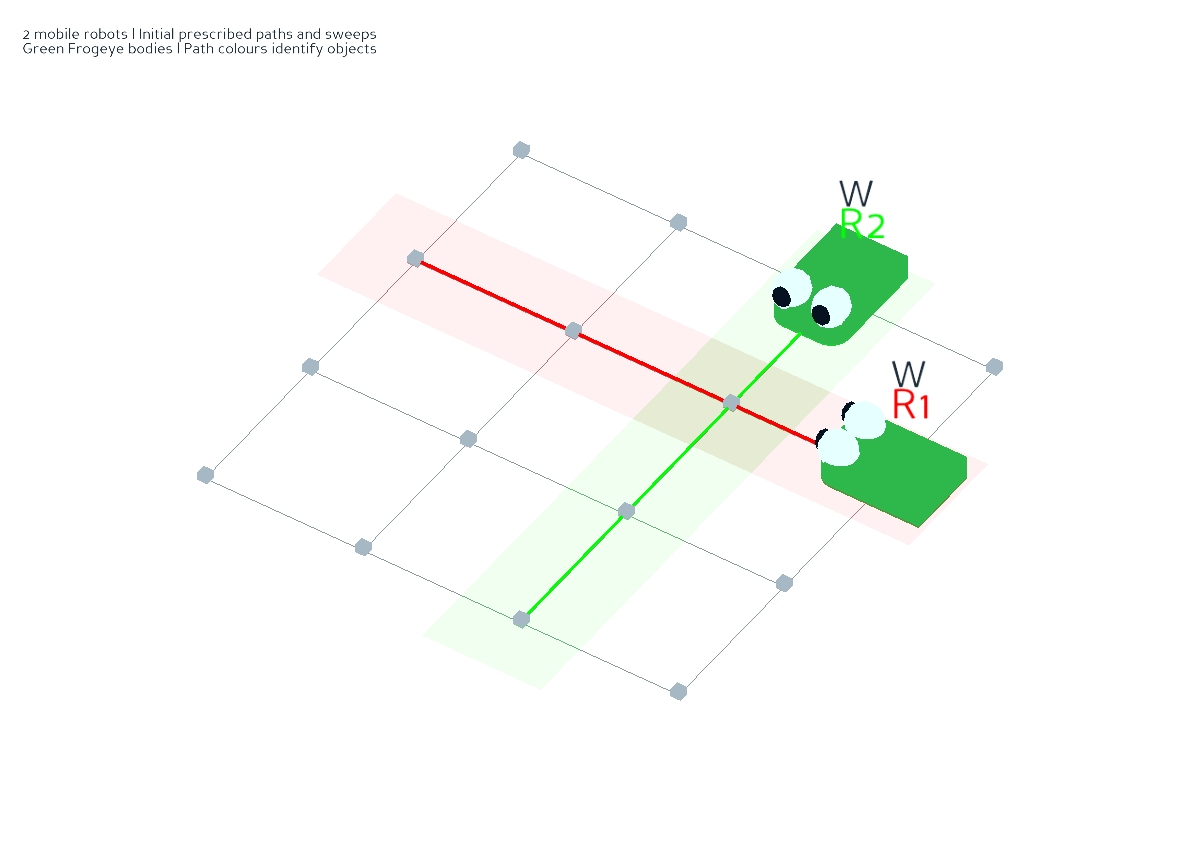
\includegraphics[width=\linewidth]{paper_02_01_RobotPath_Crossing_NoControl.png}
\par\small (a) 단일 교차 · 2대\par\scriptsize $4\times4$, $K_I=2$, $L_I=6$~m.
\end{minipage}\hfill
\begin{minipage}{.48\linewidth}\centering
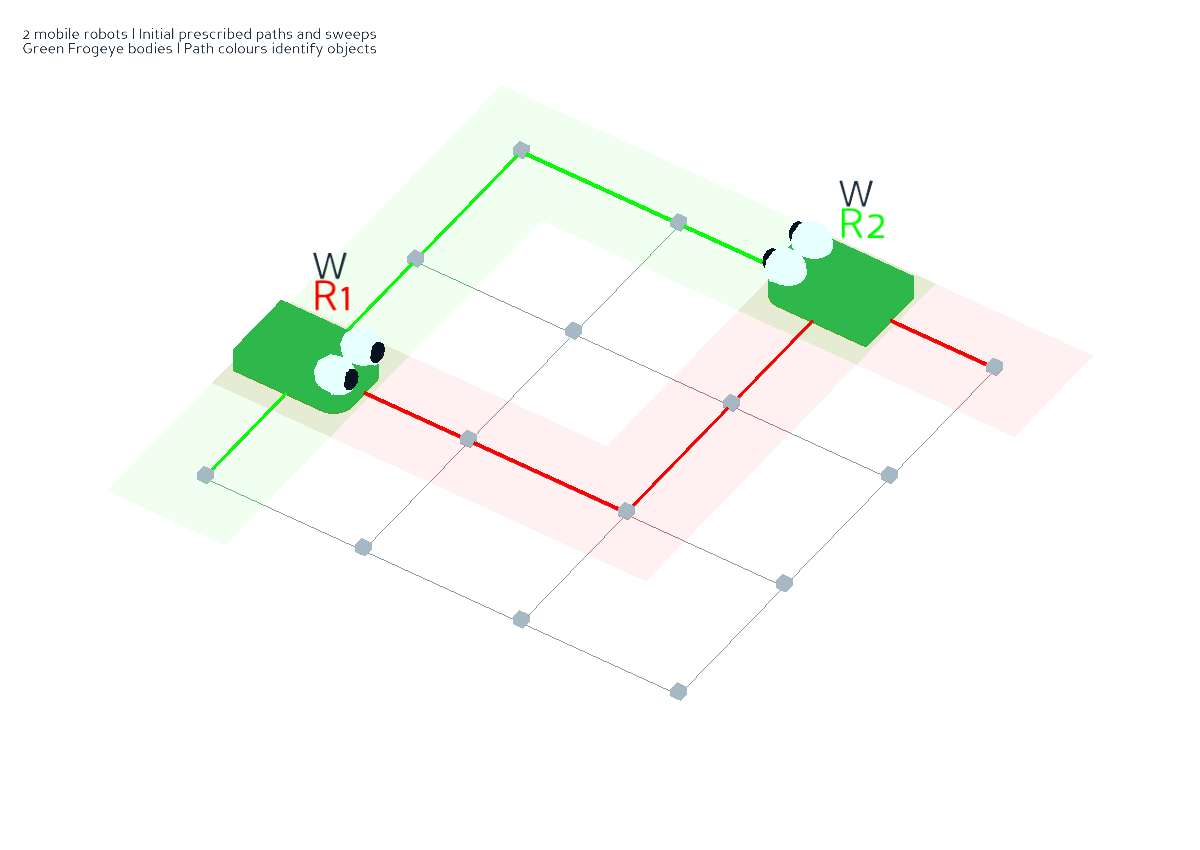
\includegraphics[width=\linewidth]{paper_02_10_RobotPath_AlternatingProgress.png}
\par\small (b) 교대 부분 진행 · 2대\par\scriptsize $4\times4$, $K_I=4$, $L_I=9$~m.
\end{minipage}\par\medskip
\begin{minipage}{.48\linewidth}\centering
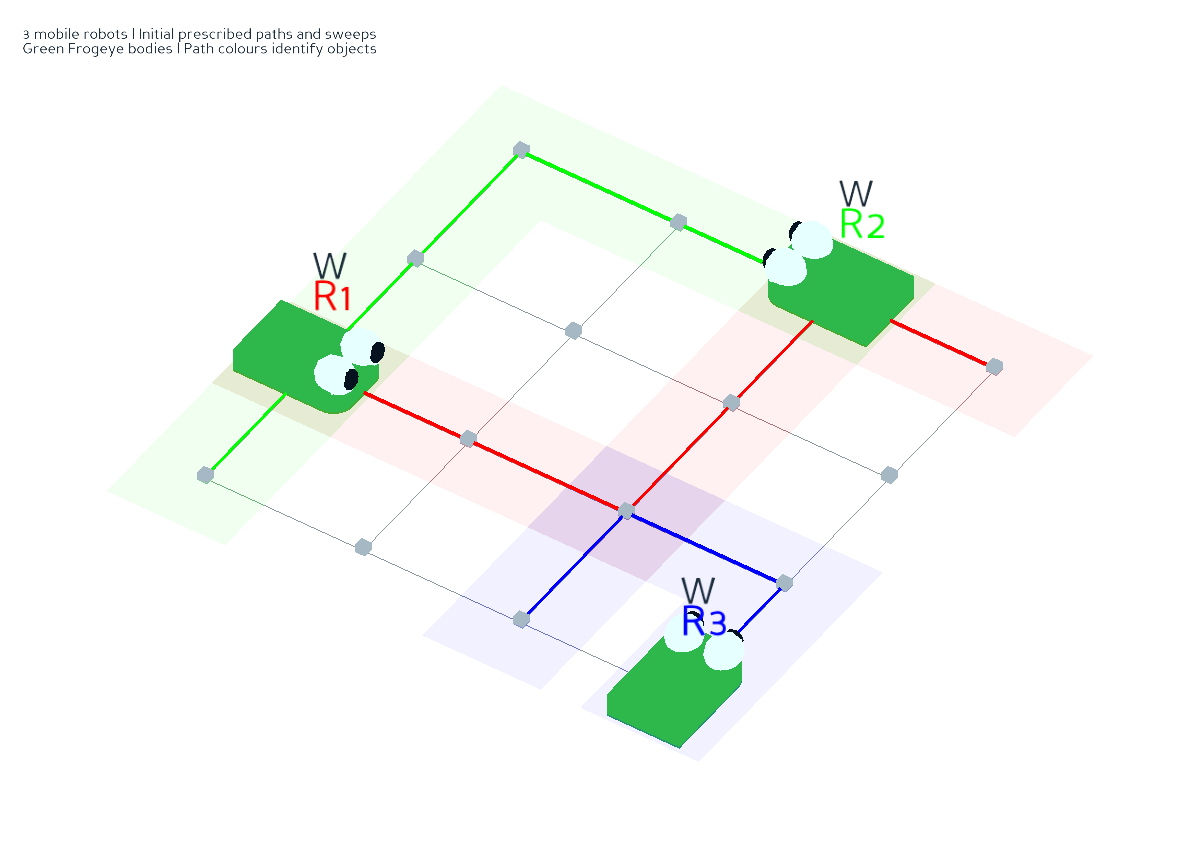
\includegraphics[width=\linewidth]{paper_03_04_RobotPath_SweepInterference.png}
\par\small (c) 전이적 간섭 · 3대\par\scriptsize $4\times4$, $K_I=6$, $L_I=15$~m.
\end{minipage}\hfill
\begin{minipage}{.48\linewidth}\centering
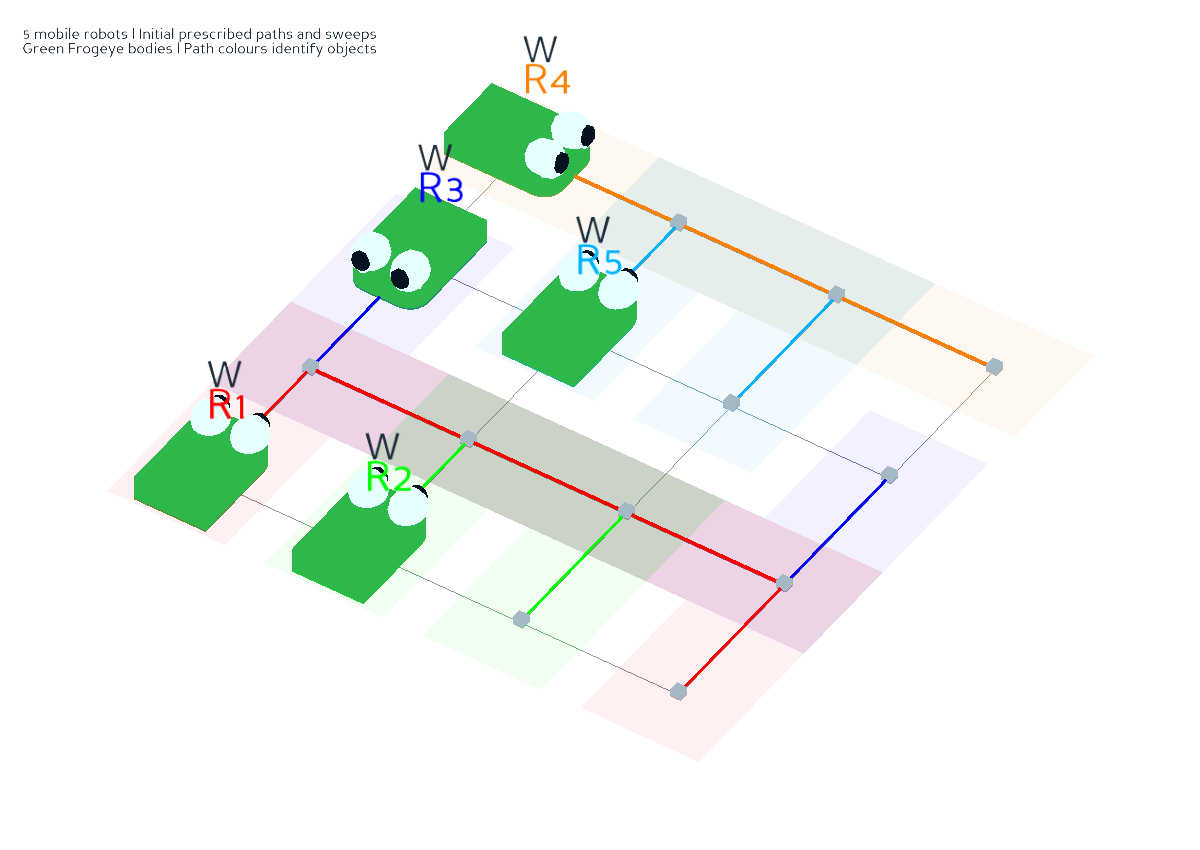
\includegraphics[width=\linewidth]{paper_05_01_RobotPath_TheoremSafeEndpoints.png}
\par\small (d) 다중 그룹 · 5대\par\scriptsize $4\times4$, $K_I=8$, $L_I=48$~m.
\end{minipage}\par\medskip
\begin{minipage}{.48\linewidth}\centering
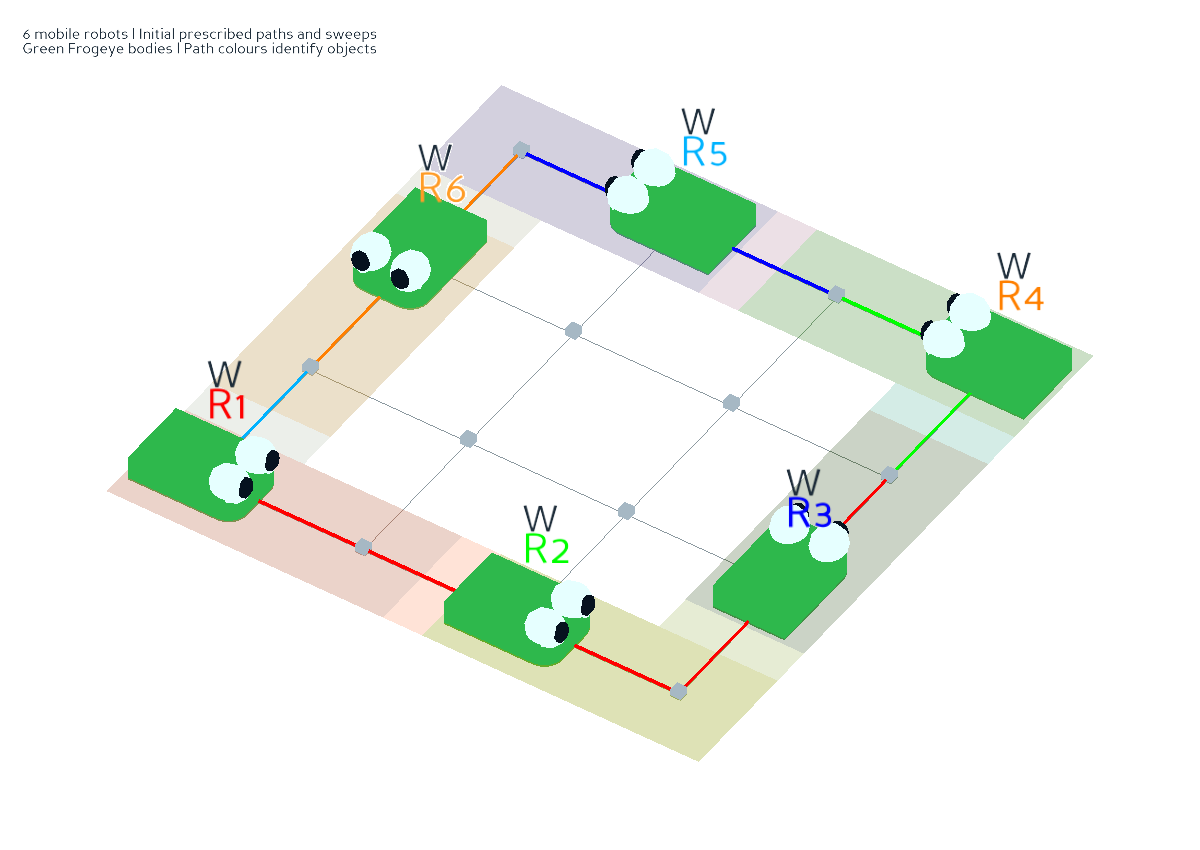
\includegraphics[width=\linewidth]{paper_06_01_RobotPath_Convoy.png}
\par\small (e) 외곽 대열 · 6대\par\scriptsize $4\times4$, $K_I=24$, $L_I=132$~m.
\end{minipage}\hfill
\begin{minipage}{.48\linewidth}\centering
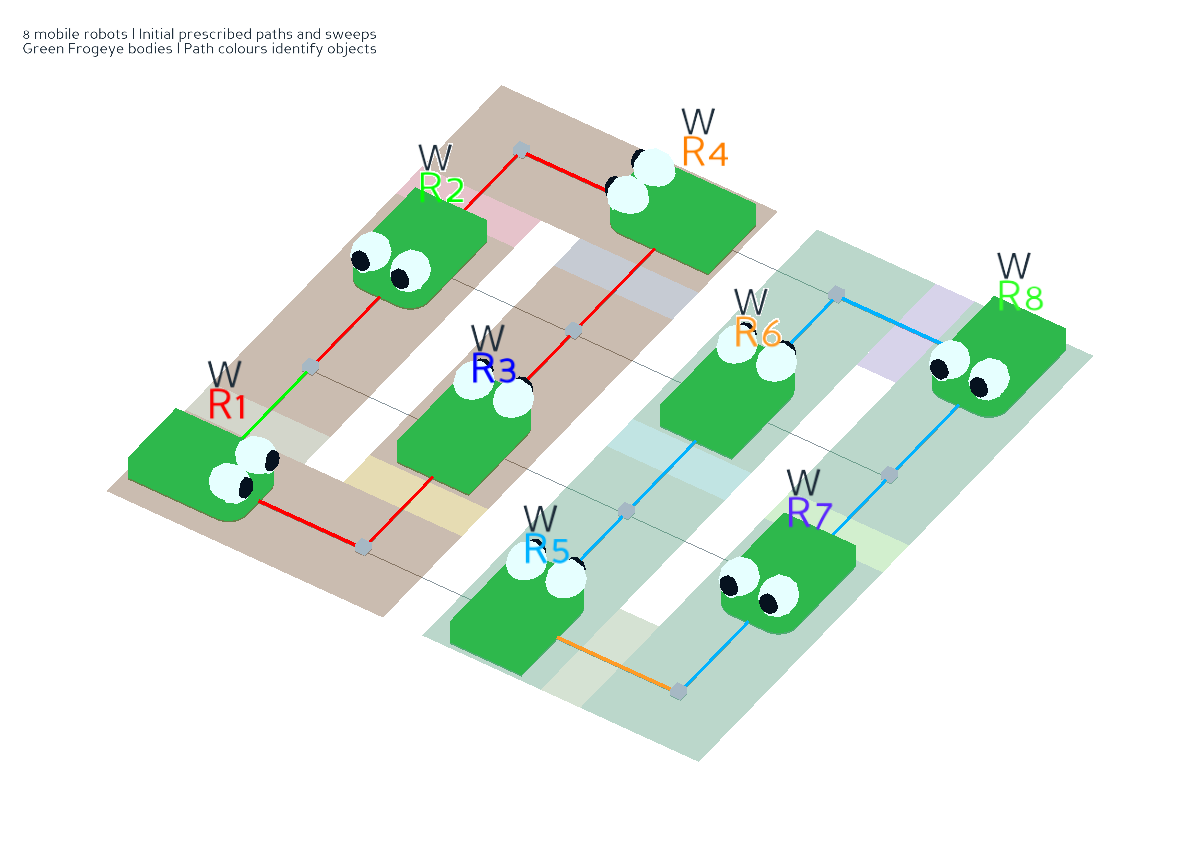
\includegraphics[width=\linewidth]{paper_08_02_RobotPath_InteriorTraffic.png}
\par\small (f) 내부 혼합 교통 · 8대\par\scriptsize $4\times4$, $K_I=24$, $L_I=336$~m.
\end{minipage}\par\medskip
\caption{예제 유형의 실제 Frogeye 뷰어 화면. 선과 반투명 스윕은 지정 경로를 나타내며 초기 스윕 겹침은 조정이 필요한 공간을 표시한다.}
\label{fig:case-gallery}
\end{figure}
\begin{figure}[p]
\centering
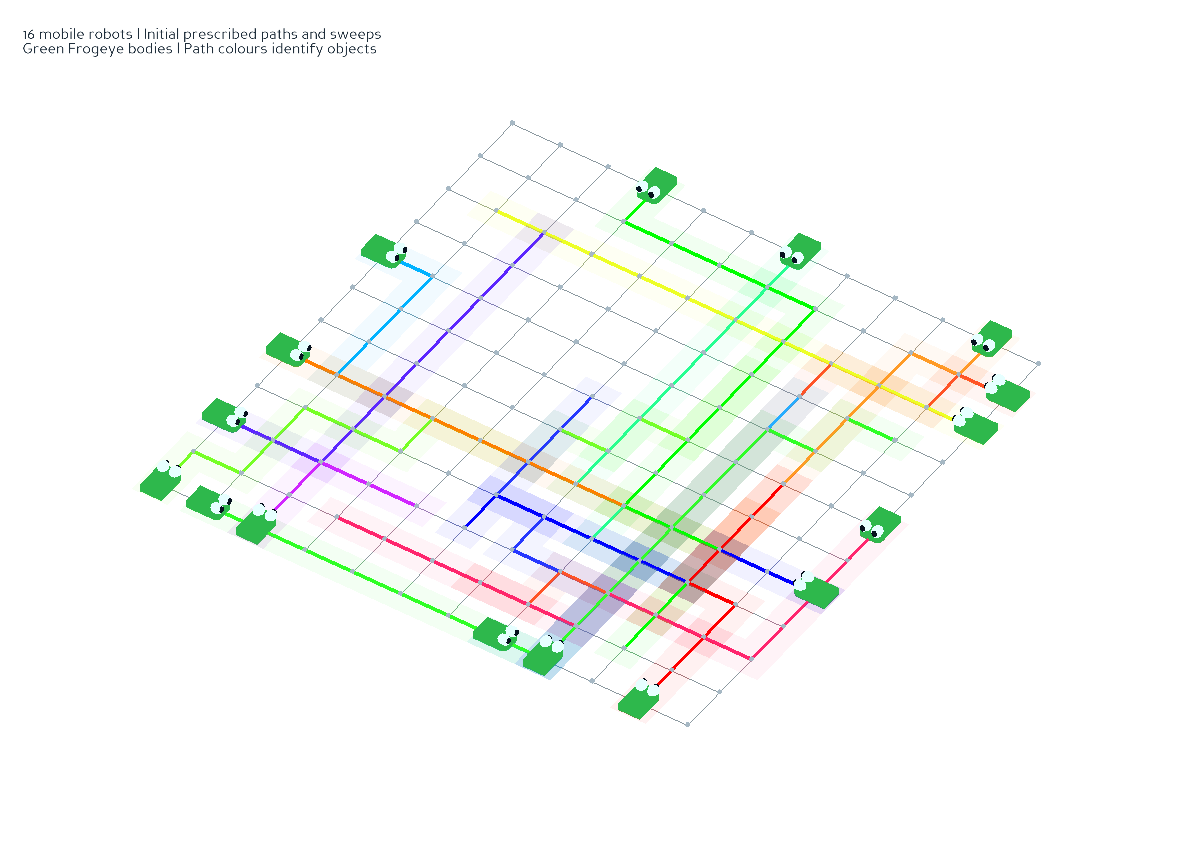
\includegraphics[width=.88\linewidth]{paper_generated_density16.png}
\par\small (a) 생성된 밀집 교통 $12\times12$, 16대,
$K_I=130$, $L_I=580.0$~m.
\par\medskip
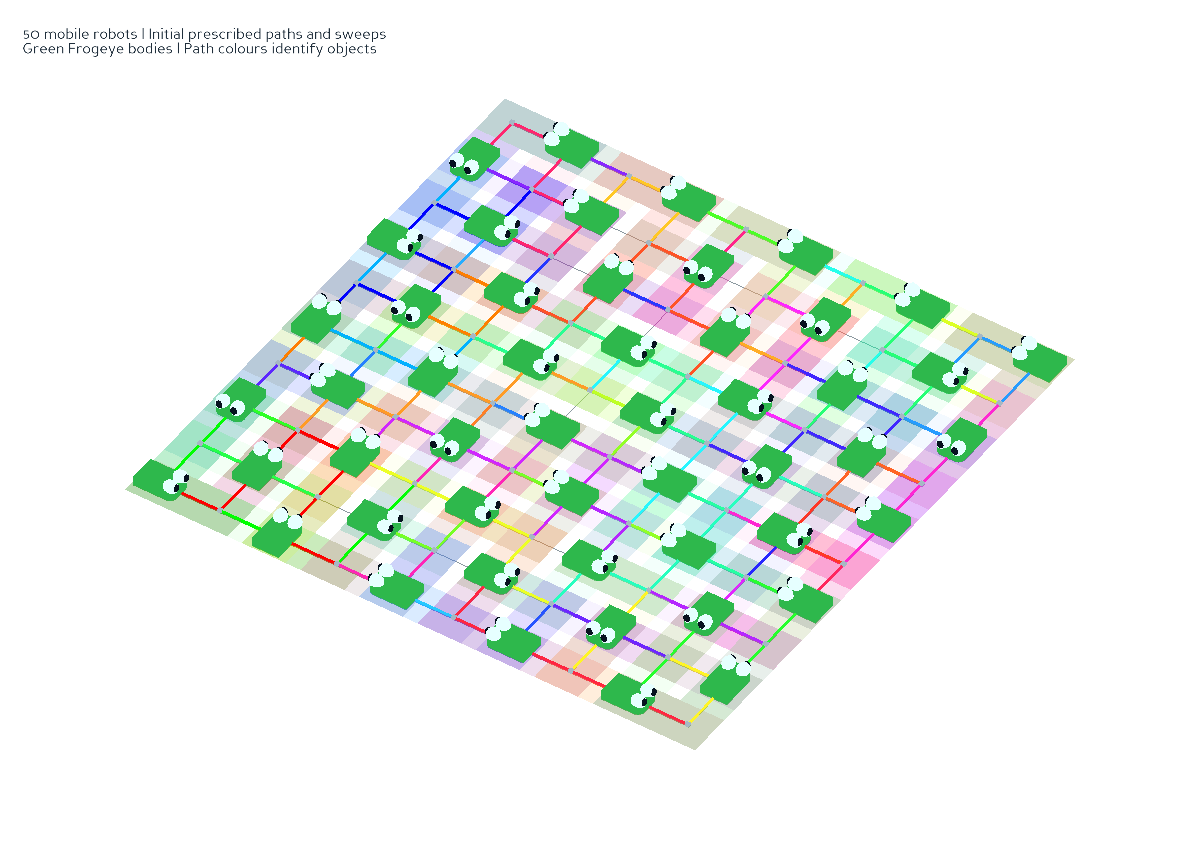
\includegraphics[width=.88\linewidth]{paper_50_01_RobotPath_InteriorTraffic.png}
\par\small (b) 내부 혼합 교통 $10\times10$, 50대,
$K_I=631$, $L_I=2581.0$~m.
\caption{실제 뷰어의 복잡한 고정 경로 예제 초기 상태. 실행 완료는 표~\ref{tab:stop-baseline-makespan}의 제어 실행으로 검증한다.}
\label{fig:dense-captures}
\end{figure}

\subsection{실행과 독립 재검증}
\ref{sec:two-policies}절의 FIFO와 LP를 적용한다. 시간 측정은 연속 및 애니메이션 간격을 무한대로 둔 DEVS 전용 실행이다. MRobot과 PSensor를 0.1~s 간격 충돌 검사 및 정지 조건으로 별도 재실행했다. 충돌은 Plant를 멈추고 검증 실패로 센다. 재실행의 명령 식별자, 로봇, 발행 시각과 완료 지표는 본 실행과 일치해야 한다.

모든 원래 작업의 완료, 활성·대기 명령 및 출력 버퍼의 소진, 모든 지정 종점에서의 MRobot Wait와 PSensor Idle, 비어 있지 않은 증거 묶음 집합으로 완료를 판정한다. 각 명령은 승인·발행·도착을 정확히 한 번 거친다. 엔진 수동 상태나 진단용 이벤트 한도만으로 완료·불가능을 판정하지 않는다. 로봇 $i$의 최종 도착이 $C_i$이면 다음을 보고한다.
\begin{equation}
 C_{\max}=\max_i C_i,\qquad \overline C=\frac1n\sum_i C_i.
 \label{eq:completion-measures}
\end{equation}
수정 후 기준 측정은 안전한 앞부분 접근, 점별 해제 및 분스합을 사용하고 목적지 연장을 끈다. 발행한 명령은 승인 종점에서 끝나야 후속 이동을 시작한다. 동일 시각에서는 0시간 제어기 명령을 먼저 전달하고, 다른 동시 자식 이벤트는 이름 순으로 처리한다.

경로 집합 13개는 3대 점검 예제 2개, 10·20·30대 각각 시드 3개 및 내부 교통 8·50대 각 1개다. 각 정책 쌍에서 경로, 초기 상태, 검증한 묶음 대안은 같고, LP는 허용된 긴 접근을 기다리는 선택과 대기자 간 최장 잔여 경로 선택을 사용한다. D10-19는 10대 DAG와 시드 20261119를 뜻하며 접미사 20·21은 20261120·20261121이다. Approach A와 Braking B는 03\_08과 03\_09 경로로, 축마다 5개 좌표인 비균일 배치에서 이동 연장을 끄고 실행했다.
\IfFileExists{Data/stop_only_baseline_tables_20261121.tex}{%
% Generated from the post-fix stop-only measurements. Do not hand-edit numbers.
\begin{table}[htbp]
\centering\small
\setlength{\tabcolsep}{4pt}
\caption{Post-fix stop-only baseline: geometry and makespan in seconds. Both policies use safe-prefix approach and sweep merging; motion extension is OFF.}
\label{tab:stop-baseline-makespan}
\begin{tabular}{rlcrrrrr}
\toprule
ID & Case & Grid & $n$ & $K_I$ & $L_I$ (m) & FIFO $C_{\max}$ & LP $C_{\max}$\\
\midrule
1 & Approach A & $5\times5$ & 3 & 4 & 12.0 & 18.394 & 18.394\\
2 & Braking B & $5\times5$ & 3 & 4 & 12.0 & 25.372 & 25.372\\
3 & D10-19 & $10\times10$ & 10 & 70 & 253.0 & 115.847 & 115.847\\
4 & D10-20 & $10\times10$ & 10 & 42 & 170.5 & 83.082 & 83.082\\
5 & D10-21 & $10\times10$ & 10 & 66 & 262.5 & 117.809 & 117.809\\
6 & D20-19 & $10\times10$ & 20 & 238 & 993.5 & 245.375 & 251.998\\
7 & D20-20 & $10\times10$ & 20 & 226 & 1002.5 & 241.505 & 241.505\\
8 & D20-21 & $10\times10$ & 20 & 220 & 872.5 & 170.859 & 170.859\\
9 & D30-19 & $12\times12$ & 30 & 398 & 1703.5 & 293.672 & 275.788\\
10 & D30-20 & $12\times12$ & 30 & 326 & 1423.0 & 217.765 & 217.765\\
11 & D30-21 & $12\times12$ & 30 & 278 & 1230.5 & 142.185 & 142.185\\
12 & Interior & $4\times4$ & 8 & 24 & 336.0 & 42.921 & 42.921\\
13 & Interior & $10\times10$ & 50 & 631 & 2581.0 & 42.921 & 42.921\\
\bottomrule
\end{tabular}
\end{table}

\begin{table}[htbp]
\centering\small
\setlength{\tabcolsep}{4pt}
\caption{Post-fix stop-only baseline: mean and population standard deviation of final path-completion times, in seconds. IDs match Table~\ref{tab:stop-baseline-makespan}.}
\label{tab:stop-baseline-mean}
\begin{tabular}{rrrrr}
\toprule
ID & FIFO $\overline C$ & FIFO $\sigma_C$ & LP $\overline C$ & LP $\sigma_C$\\
\midrule
1 & 11.627 & 4.810 & 11.627 & 4.810\\
2 & 16.043 & 6.710 & 16.043 & 6.710\\
3 & 86.301 & 28.341 & 86.301 & 28.341\\
4 & 57.574 & 19.788 & 57.574 & 19.788\\
5 & 71.034 & 34.241 & 71.034 & 34.241\\
6 & 132.145 & 60.320 & 139.351 & 69.031\\
7 & 121.958 & 69.365 & 121.958 & 69.365\\
8 & 92.432 & 50.350 & 92.432 & 50.350\\
9 & 155.324 & 79.931 & 149.002 & 73.794\\
10 & 148.591 & 43.899 & 148.591 & 43.899\\
11 & 75.321 & 34.863 & 75.321 & 34.863\\
12 & 41.921 & 1.000 & 41.921 & 1.000\\
13 & 41.561 & 1.411 & 41.561 & 1.411\\
\bottomrule
\end{tabular}
\end{table}

\begin{table}[htbp]
\centering\small
\setlength{\tabcolsep}{4pt}
\caption{Stop-only execution cost and decisions. Wall time is the median of three DEVS-only runs, excluding model/certificate construction. Stops exclude final arrivals; LP holds and waiter arbitrations are counted per execution.}
\label{tab:stop-baseline-runtime}
\begin{tabular}{rrrrrrr}
\toprule
ID & FIFO (ms) & LP (ms) & FIFO stops & LP stops & LP holds & LP selections\\
\midrule
1 & 1.32 & 1.32 & 2 & 2 & 0 & 0\\
2 & 1.27 & 1.35 & 2 & 2 & 0 & 0\\
3 & 80.03 & 79.61 & 36 & 36 & 0 & 1\\
4 & 61.21 & 62.54 & 19 & 19 & 0 & 0\\
5 & 77.34 & 74.03 & 30 & 30 & 0 & 0\\
6 & 548.64 & 557.13 & 95 & 96 & 1 & 1\\
7 & 473.45 & 475.14 & 75 & 75 & 0 & 0\\
8 & 425.76 & 426.27 & 86 & 86 & 0 & 0\\
9 & 1925.18 & 1916.71 & 154 & 154 & 1 & 1\\
10 & 1741.28 & 1715.11 & 143 & 143 & 0 & 0\\
11 & 1286.06 & 1292.60 & 126 & 126 & 0 & 0\\
12 & 25.17 & 24.91 & 48 & 48 & 0 & 0\\
13 & 1511.99 & 1471.15 & 300 & 300 & 0 & 0\\
\bottomrule
\end{tabular}
\end{table}

}{%
% Generated from the post-fix stop-only measurements. Do not hand-edit numbers.
\begin{table}[htbp]
\centering\small
\setlength{\tabcolsep}{4pt}
\caption{Post-fix stop-only baseline: geometry and makespan in seconds. Both policies use safe-prefix approach and sweep merging; motion extension is OFF.}
\label{tab:stop-baseline-makespan}
\begin{tabular}{rlcrrrrr}
\toprule
ID & Case & Grid & $n$ & $K_I$ & $L_I$ (m) & FIFO $C_{\max}$ & LP $C_{\max}$\\
\midrule
1 & Approach A & $5\times5$ & 3 & 4 & 12.0 & 18.394 & 18.394\\
2 & Braking B & $5\times5$ & 3 & 4 & 12.0 & 25.372 & 25.372\\
3 & D10-19 & $10\times10$ & 10 & 70 & 253.0 & 115.847 & 115.847\\
4 & D10-20 & $10\times10$ & 10 & 42 & 170.5 & 83.082 & 83.082\\
5 & D10-21 & $10\times10$ & 10 & 66 & 262.5 & 117.809 & 117.809\\
6 & D20-19 & $10\times10$ & 20 & 238 & 993.5 & 245.375 & 251.998\\
7 & D20-20 & $10\times10$ & 20 & 226 & 1002.5 & 241.505 & 241.505\\
8 & D20-21 & $10\times10$ & 20 & 220 & 872.5 & 170.859 & 170.859\\
9 & D30-19 & $12\times12$ & 30 & 398 & 1703.5 & 293.672 & 275.788\\
10 & D30-20 & $12\times12$ & 30 & 326 & 1423.0 & 217.765 & 217.765\\
11 & D30-21 & $12\times12$ & 30 & 278 & 1230.5 & 142.185 & 142.185\\
12 & Interior & $4\times4$ & 8 & 24 & 336.0 & 42.921 & 42.921\\
13 & Interior & $10\times10$ & 50 & 631 & 2581.0 & 42.921 & 42.921\\
\bottomrule
\end{tabular}
\end{table}

\begin{table}[htbp]
\centering\small
\setlength{\tabcolsep}{4pt}
\caption{Post-fix stop-only baseline: mean and population standard deviation of final path-completion times, in seconds. IDs match Table~\ref{tab:stop-baseline-makespan}.}
\label{tab:stop-baseline-mean}
\begin{tabular}{rrrrr}
\toprule
ID & FIFO $\overline C$ & FIFO $\sigma_C$ & LP $\overline C$ & LP $\sigma_C$\\
\midrule
1 & 11.627 & 4.810 & 11.627 & 4.810\\
2 & 16.043 & 6.710 & 16.043 & 6.710\\
3 & 86.301 & 28.341 & 86.301 & 28.341\\
4 & 57.574 & 19.788 & 57.574 & 19.788\\
5 & 71.034 & 34.241 & 71.034 & 34.241\\
6 & 132.145 & 60.320 & 139.351 & 69.031\\
7 & 121.958 & 69.365 & 121.958 & 69.365\\
8 & 92.432 & 50.350 & 92.432 & 50.350\\
9 & 155.324 & 79.931 & 149.002 & 73.794\\
10 & 148.591 & 43.899 & 148.591 & 43.899\\
11 & 75.321 & 34.863 & 75.321 & 34.863\\
12 & 41.921 & 1.000 & 41.921 & 1.000\\
13 & 41.561 & 1.411 & 41.561 & 1.411\\
\bottomrule
\end{tabular}
\end{table}

\begin{table}[htbp]
\centering\small
\setlength{\tabcolsep}{4pt}
\caption{Stop-only execution cost and decisions. Wall time is the median of three DEVS-only runs, excluding model/certificate construction. Stops exclude final arrivals; LP holds and waiter arbitrations are counted per execution.}
\label{tab:stop-baseline-runtime}
\begin{tabular}{rrrrrrr}
\toprule
ID & FIFO (ms) & LP (ms) & FIFO stops & LP stops & LP holds & LP selections\\
\midrule
1 & 1.32 & 1.32 & 2 & 2 & 0 & 0\\
2 & 1.27 & 1.35 & 2 & 2 & 0 & 0\\
3 & 80.03 & 79.61 & 36 & 36 & 0 & 1\\
4 & 61.21 & 62.54 & 19 & 19 & 0 & 0\\
5 & 77.34 & 74.03 & 30 & 30 & 0 & 0\\
6 & 548.64 & 557.13 & 95 & 96 & 1 & 1\\
7 & 473.45 & 475.14 & 75 & 75 & 0 & 0\\
8 & 425.76 & 426.27 & 86 & 86 & 0 & 0\\
9 & 1925.18 & 1916.71 & 154 & 154 & 1 & 1\\
10 & 1741.28 & 1715.11 & 143 & 143 & 0 & 0\\
11 & 1286.06 & 1292.60 & 126 & 126 & 0 & 0\\
12 & 25.17 & 24.91 & 48 & 48 & 0 & 0\\
13 & 1511.99 & 1471.15 & 300 & 300 & 0 & 0\\
\bottomrule
\end{tabular}
\end{table}

}

\subsection{수정 후 정차 방식 기준 결과}
13개 경로의 26개 정책 조건에서 시간 측정 실행 78회와 충돌 정지 재실행 26회를 모두 완료했으며 재실행의 검출 접촉은 0회다. 로봇별 완료시간과 연장 횟수의 반복 일치를 확인했고, 연장 명령은 모든 조건에서 0회였다. 모집단 표준편차는 사례 내 로봇 간 차이다. 실행 비용 표는 세 번의 중앙값으로 입력·증거 구성, 렌더 및 재실행을 제외한다.

LP의 전체 완료시간은 한 사례에서 더 짧고 한 사례에서 더 길며 11개에서 같았다. 평균 완료시간도 같은 방향이었다. LP의 의도적 대기는 두 번 기록되었다. 이동 연장의 효율을 보려면 이 기준 조건과 짝지어 재실행해야 한다. 이 검증은 구현의 묶음 지원 및 점유 조건을 다룬다. 완료 보장은 명시한 가정을 따르며 표본 충돌 검사는 연속시간 증명과 구별한다.

\subsection{랙을 든 20대의 창고 배치}
\label{sec:warehouse}
비균일 간격의 통로 그래프에 정점 401개, 양방향 링크 527개, 작업대 10개, 랙 셀 120개를 둔다. 구현은 축 정렬 평면 구간과 직사각형 외곽을 사용한다. 고정 경로 집합 5개에 각각 20대의 랙 운반 로봇을 둔다. 10대는 랙 셀에서 작업대로, 10대는 작업대 앞에서 반품 랙 셀로 향한다. 이동용으로 20개 셀을 비워 정지 랙 100개를 남긴다. 거리 가중 A*로 사전에 경로를 생성하고 쌍별 실행 가능성과 비순환 요구 그래프를 검사했다. 전체 주문 주기와 구분한 고정 경로 실험이며, 코너에서 로봇 본체가 회전해도 랙 방향은 유지한다.
\begin{figure}[p]
\centering
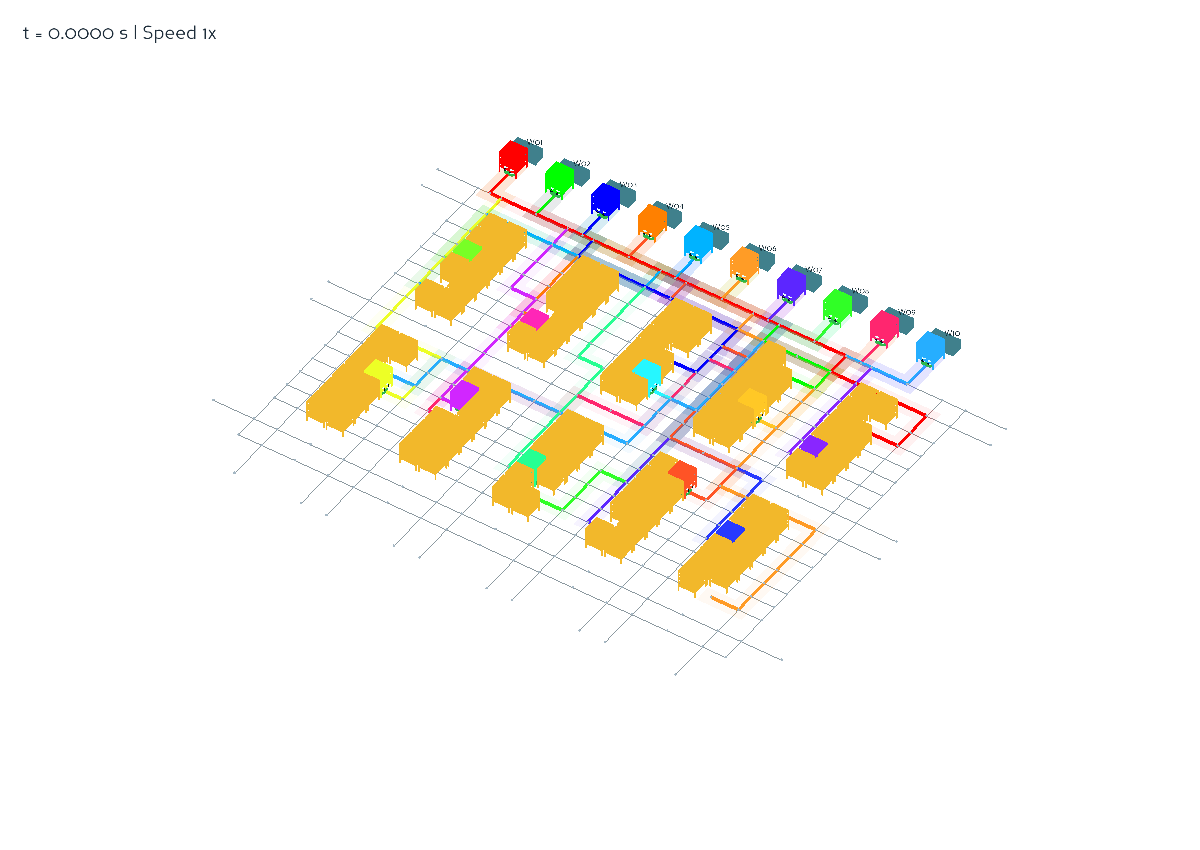
\includegraphics[width=.94\linewidth,trim=90 100 90 70,clip]{warehouse20_iso_initial.png}
\par\smallskip (a) 초기 배치와 지정 경로, $t=0$ s.
\par\medskip
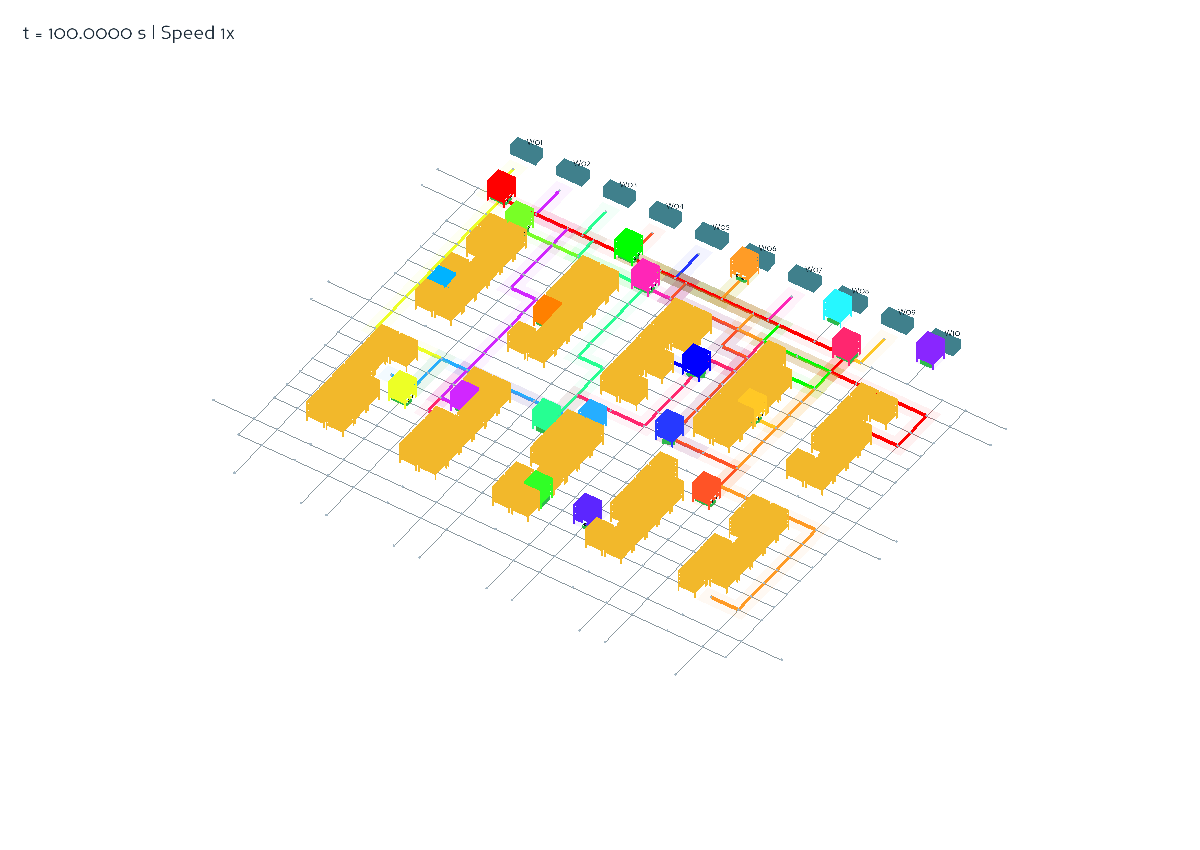
\includegraphics[width=.94\linewidth,trim=90 100 90 70,clip]{warehouse20_iso_progress.png}
\par\smallskip (b) FIFO 실행과 잔여 경로, $t=100$ s.
\caption{창고 집합 1의 실제 Iso 화면. 색상이 지정된 이동 랙은 20대의 로봇에 대응한다. 노란 랙은 정지 상태이며 물리 진행 보고로 지난 경로 영역을 해제한다.}
\label{fig:warehouse-iso}
\end{figure}
\begin{table}[htbp]
\centering\small
\caption{랙을 든 20대와 고정 경로 집합 5개의 이전 실험. 시간 단위는 초다. $K_I$와 $L_I$는 표~\ref{tab:stop-baseline-makespan}과 같은 방향성 간섭 정의를 사용한다.}
\label{tab:warehouse-results}
\begin{tabular}{rrrrrrr}
\toprule
집합 & $K_I$ & $L_I$ (m) & \multicolumn{2}{c}{FIFO} & \multicolumn{2}{c}{LP}\\
 & & & $C_{\max}$ & 평균 & $C_{\max}$ & 평균\\
\midrule
1 & 252 & 1769.30 & 522.25 & 243.79 & 522.25 & 243.79\\
2 & 266 & 1756.48 & 413.24 & 216.81 & 413.24 & 216.81\\
3 & 310 & 2242.88 & 540.70 & 288.15 & 540.70 & 288.43\\
4 & 266 & 1696.35 & 359.65 & 197.50 & 359.65 & 197.50\\
5 & 256 & 1655.63 & 343.69 & 193.24 & 343.69 & 193.24\\
\bottomrule
\end{tabular}
\end{table}
본 실행 10회와 0.01~s 충돌 정지 재실행 10회를 모두 완료했으며 접촉 검출은 없었다. 명령 이력이 일치했고 경로 생성 단계에서 고정 랙과의 분리를 검사했다. 모든 집합에서 FIFO와 LP의 makespan은 같고 집합 3만 평균 완료시간이 달랐다.
\begin{quote}\small\ttfamily
python -m examples.RMFS.Tests.20\_04\_RobotPath\_WarehouseExchange\\
\hspace*{1em}--case 1 --policy fifo --fps 10 --non-interactive
\end{quote}
사례는 1--5, 정책은 \texttt{fifo} 또는 \texttt{lp}다. 결과는 \path{Tests/results/warehouse20_validation.json}에 있다. 검증은 모듈 \path{examples.RMFS.Tests.run_warehouse_paths}에 \texttt{--validate}를 전달해 재현한다. 이전 검증은 86개 사례, 본 실행 172회와 재실행 172회를 포함하며 최신 정차 기준과 구분한다.

\section{결과 평가와 산업적 관련성}
\label{sec:contributions}
\paragraph{선행연구와 대조한 기여}
\ref{sec:prior-art}절의 대응에서 스윕 양립, 대기 삽입, 부분 진행과 선행 기반 실행은 기존 원리다. 1989년 연구는 종점 차단과 전체 경로 순차 실행을 넘어선 조정을 다뤘고, SCALE은 더 넓은 계획·실행을 결합했다. 본 논문의 정의와 증명은 특수 정식화와 구현을 설명한다.

\subsection{정규 격자가 필요 없는 기하 간섭}
점유 스윕으로 간섭을 정의하므로 비균일 간격과 일반 경로 그래프에도 추상 묶음 및 실행 조건을 적용한다. 창고 예제의 401개 정점과 527개 링크에서 이를 확인했다. 실제 경로는 축 정렬이며 임의 곡선과 일반 3D 스윕은 구현 범위 밖이다. 랙 및 통로 형상이 셀 분할에 일치하지 않을 때 이 구분이 유용하며 안전한 기하 외곽은 계속 필요하다. 비격자 조정은 선행연구에도 있다.
\begin{table}[htbp]
\centering\small
\caption{기존 연구의 성질과 본 구현의 비교.}
\label{tab:literature-comparison}
\begin{tabular}{p{.22\linewidth}p{.34\linewidth}p{.35\linewidth}}
\toprule
비교 항목 & 선행 접근법 & 본 논문의 구현\\\midrule
간섭 표현 & 구간 스윕~\cite{odonnell1989}, 기하학적 조정~\cite{leroy1999}, 이종 스윕~\cite{scale2026} & 정규 격자를 전제하지 않는 고정 직사각형 스윕.\\[4pt]
일정 구성 & 구간 진행 탐색과 종점 차단~\cite{odonnell1989} & 점 토큰과 대기 탐색. 식~\eqref{eq:prior-progress} 참조.\\[4pt]
기하 비용 & 조정 도표~\cite{leroy1999}, 적응적 여유 질의~\cite{ablad2021} & 2차원 직사각형 구간 스윕.\\[4pt]
실행 & 우선순위와 의존성 기반 안전 실행 및 병합~\cite{gregoire2015,cap2016,hoenig2019,berndt2024,scale2026} & 검증 묶음, 원래 작업의 순서, 허가된 병합 및 보고 기반 해제.\\[4pt]
시연 & 서로 다른 기하, 대수와 작업 부하. & 수정 후 FIFO/LP 13개 경로 집합, 최대 50대. 이전 창고 및 설명 실험은 별도.\\
\bottomrule
\end{tabular}
\end{table}

\subsection{스윕 제어의 계산 가능한 구현}
고정 방향 직사각형이라는 형상과 운동을 선택하고 의미 있는 보고를 받아 지나간 공간을 해제한다. 스윕은 선택 형상에 대해 정확하며 형상 자체는 실제 본체와 하중을 근사한다. DEVS Plant에서 가속·정속·감속·회전을 예약하고, 일정 간격 출발 검사 없이 제어한다. 한 명령으로 합쳐도 허가를 위해 원래 작업을 유지한다.

\paragraph{시간을 포함한 실행과 상호작용 애니메이션}
이벤트 제어를 3D Plant와 결합하고 $1\times$에서 실시간 속도의 재생을 목표로 한다. 화면 샘플링과 제어 이벤트는 역할이 다르며 같은 모델을 사용한다. 그림~\ref{fig:warehouse-iso}는 창고의 Iso 화면이다. 50대 화면에 렌더 부하가 관찰됐으므로 프레임률이나 실시간 마감 보장에 대한 근거로 사용하지 않는다.

\paragraph{시뮬레이션 계산시간}
표~\ref{tab:realtime-evidence}의 50대 헤드리스 실행은 두 정책 모두 시뮬레이션 42.92초를 설정 포함 실제 10초 미만에 마쳐 해당 장비에서 약 4.5배 빨랐다. 경로 생성과 외부 작업 준비는 측정 전이며 렌더 및 별도 충돌 재실행은 제외했다.
\begin{table}[htbp]
\centering\small
\caption{최근 수정 전 50대 내부 교통의 헤드리스 실행 시간. 최신 실행 전용 중앙값은 표~\ref{tab:stop-baseline-runtime}에 있다. 아래는 설정을 포함한 개별 실행이며 렌더링과 샘플 충돌 검사는 제외한다.}
\label{tab:realtime-evidence}
\begin{tabular}{lrrrr}
\toprule
정책 & 모의 시간(s) & 설정(s) & 실제 시간(s) & 시간 비\\
\midrule
FIFO & 42.92 & 1.15 & 9.62 & 4.46\\
LP   & 42.92 & 1.12 & 9.56 & 4.49\\
\bottomrule
\end{tabular}
\end{table}
이 계산시간은 해당 입력의 실행 가능성을 뒷받침한다. 하드웨어와 작업이 다른 기존 연구의 속도 비교나 일반 확장 법칙에는 대수 외에도 간섭 수, 총간섭 길이와 연결성을 고려해야 한다.

\subsection{RMFS 모델링과 제어에 대한 기여}
첫째, 명시한 완료 조건 아래 스윕과 순서 성질을 사용해 고정 경로의 무충돌 제어를 구성한다. 점 대기와 허용 병합은 순서를 유지한다. 새 기준 실험은 13개 경로 집합에서 FIFO와 LP를 시간 측정 반복 3회와 독립 재실행으로 검증했다. 이전 창고 및 설명 실험은 별도로 표시한다.

둘째, 후보 경로를 개별 거리뿐 아니라 잔여 스윕과 완료 조건으로 평가하는 간섭 고려 경로 생성의 토대가 된다. RobotPathPlanner는 시간 목적에 따라 실행 가능한 경로를 비교할 수 있다. 생성·최적화 알고리즘과 평가는 후속 연구다. 공학적으로 확인 가능한 예약, 해제 보고와 랙 운반 로봇 실험을 제공하며 실제 배치에는 위치 오차·통신 지연·정차 불확실성을 반영한 외곽과 피드백 여유가 필요하다.

\section{재현 방법과 한계}
\label{sec:reproducibility}
\subsection{저장소와 독자 접근}
소스 저장소는 다음과 같다.
\begin{center}
\url{https://github.com/mhhwang2002/SOCS}.
\end{center}
이 절의 경로는 저장소 루트 기준이다. 구현 및 예제는 \nolinkurl{examples/RMFS}, 단위 테스트는 \nolinkurl{tests/examples/RMFS}에 있다. 두 원고는 다음 논문 디렉터리에 있다.\par
\nolinkurl{docs/RMFS/Papers/2026_11_SweepBasedCollisionAvoidanceFramework/}\par
영문과 한글 원고의 파일명은 각각 다음과 같다.
\begin{quote}\small
\nolinkurl{SweepBasedCollisionAvoidanceFramework_en.tex}\par
\nolinkurl{SweepBasedCollisionAvoidanceFramework_kr.tex}
\end{quote}

독자가 제한 없이 읽으려면 저장소나 재현용 미러가 공개되어 있어야 한다. 공개 저장소는 쓰기 권한 없이 복제할 수 있으며, 비공개 저장소는 별도 접근 권한이 필요하다.\footnote{GitHub의 \href{https://docs.github.com/en/repositories/creating-and-managing-repositories/about-repositories}{저장소 공개 범위 안내}를 참조한다.} 새 산출물을 독자가 받으려면 커밋 및 푸시해야 한다. 출판 전에 불변 커밋 또는 릴리스 태그를 인용한다. 이 연구 원고에는 릴리스 식별자가 확정되지 않았다.

\subsection{환경 설정}
Python 3.13 이상이 필요하다. Panda3D는 애니메이션을 제공하며 개발용 추가 패키지는 회귀 테스트용 pytest를 설치한다. 저장소를 복제한 뒤 가상 환경을 만든다.
\begin{quote}\small
\begin{verbatim}
git clone https://github.com/mhhwang2002/SOCS.git
cd SOCS
python -m venv .venv
\end{verbatim}
\end{quote}
Windows PowerShell에서는 다음으로 활성화한다.
\begin{quote}\small
\begin{verbatim}
.\.venv\Scripts\Activate.ps1
\end{verbatim}
\end{quote}
macOS/Linux에서는 다음을 사용한다.
\begin{quote}\small
\begin{verbatim}
source .venv/bin/activate
\end{verbatim}
\end{quote}
설치 환경에 따라 \nolinkurl{python3}로 가상 환경을 생성한다. 활성화 후 편집 가능 모드로 설치한다.
\begin{quote}\small
\begin{verbatim}
python -m pip install -e ".[dev]" panda3d
\end{verbatim}
\end{quote}
보고한 실험은 Windows에서 실행했다. 다른 셸의 활성화 명령은 해당 운영체제에서 모든 예제를 검증했다는 뜻이 아니다. 아래 명령은 모두 저장소 루트에서 실행한다.

\subsection{보고된 사례 실행과 재현}
최신 정차 기준의 재현 명령은 다음과 같다.
\begin{quote}\small\begin{verbatim}
python -m examples.RMFS.Tests.run_release_extension_comparison --stop-only
python -m examples.RMFS.Tests.write_stop_baseline_tables
\end{verbatim}\end{quote}
첫 명령은 FIFO와 LP에 대해 승인 종점 정차 조건으로 DEVS 실행을 세 번 반복하고 0.1초 충돌 정지 검증을 수행한다. 둘째 명령은 \nolinkurl{examples/RMFS/Tests/results/stop_only_baseline_20261121.json}에서 원고 표를 생성한다. 같은 위치의 CSV에 사례별 지표가 있다. JSON은 경로, 입력 지문, 소스 해시, 개별 실행 및 완료 시각, 검증 상태를 보존한다. \nolinkurl{paper_fifo_lp_final.json} 같은 과거 자료는 최신 기준표와 별개다.

경로 데이터는 \nolinkurl{examples/RMFS/Tests/data/generated/}에 있다. \texttt{density12} 하위 폴더의 \texttt{objects\_4.json}, \texttt{objects\_8.json}, \texttt{objects\_12.json}, \texttt{objects\_16.json}과 별도 계열의 \texttt{complex.json}, \texttt{random\_trial.json}은 시드, 생성 인수, 기하, 끝점 검사 및 검증 묶음을 저장한다. \texttt{generate\_path\_data --help}로 생성 매개변수를 확인하며 경로 채택에 실행 완료시간은 사용하지 않는다.

실제 뷰어 초기 화면은 \nolinkurl{examples/RMFS/Tests/capture_paper_examples.py}로 캡처한다.
\begin{quote}\small\begin{verbatim}
python -m examples.RMFS.Tests.capture_paper_examples `
  --case 03_04_RobotPath_SweepInterference `
  --output three_objects.png
\end{verbatim}\end{quote}
PowerShell의 백틱은 줄 연결이며 다른 셸에서는 한 줄로 합친다. \texttt{NoControl}이나 \texttt{Collision}이 포함된 예제 이름은 과거의 무제어 시연을 보존한다. 본문의 제어 실행은 위 검증 절차를 따른다.

제어된 2·3대 애니메이션은 \nolinkurl{run_framework_paper_examples}에 \texttt{--case 2} 또는 \texttt{--case 3}을 주어 실행한다. 같은 기하의 단일 기준 묶음 제어를 시각화한다. 뷰어에서 A는 자동/수동, Space는 한 이벤트 진행, R은 초기화, T/I는 Top/Iso, U/D는 속도, Esc는 닫기다. 기본 배경은 흰색이다.

유한 끝점 분류는 다음으로 재현한다.
\begin{quote}\small\begin{verbatim}
python -m examples.RMFS.Tests.run_unit_pair_classification --max-edges 5
\end{verbatim}\end{quote}
제한된 유한 분류다. 정책 정의 및 피드백 테스트는 \nolinkurl{tests/examples/RMFS}의 \nolinkurl{test_paper_policy_definition.py}, \nolinkurl{test_fifo_traffic.py}, \nolinkurl{test_event_release.py}에 있다.

\subsection{한계}
\begin{enumerate}
\item 작업 기반 정확성은 Plant와 피드백 가정 아래의 증명 개요이며 수치 구현의 형식 검증은 범위 밖이다.
\item 정적 비순환 요구 조건은 실행 가능한 일부 순환도 배제한다.
\item 안전 여유, 통신 지연, 위치 오차, 돌발 장애물, 물리 정지 거동은 별도 분석이 필요하다.
\item 유한 분류와 성능 실험의 결론은 명시한 영역과 지표에 적용된다.
\item 새로운 조정 원리를 주장하려면 선행연구와 더 깊은 기술 비교가 필요하다.
\end{enumerate}

\section{결론과 후속 연구 범위}
본 논문은 기존 스윕 기반 조정 원리를 이벤트 기반 이동 제어에 연결했다. 완전한 묶음경로는 이동과 대기를 나타내며, 안전한 분스합은 원래 제어 단위를 보존한다. 보수적 해제로 공유 RoadMap을 갱신한다. 제시한 명제는 명시된 기하, 피드백 및 실행 가정 아래 안전과 유한시간 완료를 보인다. FIFO와 LP는 그 조건 안에서 동작을 선택한다. 영역 기반 정식화는 일반적이며, 구현과 수치 실험은 2차원 직사각형 외곽을 대상으로 한다.

정차 기준은 3대 점검부터 50대 내부 교통까지 13개 경로 집합의 두 정책 모두에서 완료했다. 조건마다 시간 측정을 세 번 반복하고 별도 충돌 정지 재실행을 일치시켰다. 완료 지표와 함께 간섭 구간 수와 길이를 보고했다. 이 결과는 사례에 대한 구현 검증이며 이론적 보장은 별도로 명시한 가정을 따른다.

공학적 결과는 명시한 완료 조건 아래 주어진 경로를 무충돌로 제어한 것이다. 현재 위치, 목적지, 잔여 스윕에서 RobotPathPlanner가 후보 경로를 검사하고 시간 기반 완료 목적을 평가할 수 있다. 간섭을 고려한 최적 경로 생성과 평가는 후속 연구다.

\paragraph{시간 기반 진입과 안전한 순서 수정}
Coskun과 O'Kane의 시간 기반 순서 수정~\cite{coskun2019}과 Segment Graph의 교착 검사~\cite{coskun2021}를 TrafficManager에 적용해 비교할 수 있다. 잔여 스윕이 겹쳐도 한 로봇이 다른 로봇의 진입 전에 공유 구역을 비울 수 있어 보수적 제어에 대기가 생긴다. 가감속 및 회전 모델로 해제와 진입을 추정하고, 전역 의존성, 종점 점유와 실제 Plant 해제 피드백을 검증한 뒤 예약을 갱신해야 한다. 대기, 완료시간, 계산비용, 충돌 및 교착을 지연과 하류 차단이 있는 사례에서 비교한다. 예상 시각만으로 안전을 보장할 수 없다.

정차 상태에서 평가하는 lookahead와 감속 전에 주행 상태에서 평가하는 lookahead의 차이는 후속 연구 변수다. \ref{sec:prebraking-review}절에서 감속 경계 이벤트, 시뮬레이션 기반 진입 허가, 제동선 제어의 선행연구를 정리했다. 직접 대조에서 두 로봇의 유한 구성은 고전 구간 진행 조정에 대응하고 기존 동작 그래프가 교대 진행 예제를 표현할 수 있으며, SCALE은 더 넓은 통합 기능을 다룬다. 향후 경로 생성의 기여는 별도의 방법과 증거로 평가한다.

본 논문은 명시된 가정 아래 고정 경로의 충돌 회피와 완료를 다룬 것으로 마무리한다. 별도 연구에서는 정차 후 허가와 Push/Pull 제어를 비교한다. 감속 전 요청과 검증된 공간 해제에 따라 이동 프로파일을 연장한다. 동일한 경로와 통과 순서에서 로봇 본체, 랙 및 적재물의 질량을 따로 모델링하고 총 배터리 소비 에너지와 전체 완료시간을 평가한다. 에너지 절감과 두 지표의 공동 최적화는 후속 연구의 목표다.

{\latinfont
\begin{thebibliography}{99}

\bibitem{zeigler1976}
B.~P. Zeigler.
\newblock \emph{Theory of Modelling and Simulation}.
\newblock First edition. Wiley-Interscience, New York, 1976.

\bibitem{zeigler2018}
B.~P. Zeigler, A. Muzy, and E. Kofman.
\newblock \emph{Theory of Modeling and Simulation: Discrete Event \& Iterative
System Computational Foundations}.
\newblock Third edition. Academic Press, 2018.
\newblock \url{https://doi.org/10.1016/C2016-0-03987-6}.

\bibitem{odonnell1989}
P.~A. O'Donnell and T. Lozano-P\'erez.
\newblock Deadlock-free and collision-free coordination of two robot manipulators.
\newblock In \emph{Proceedings of the IEEE International Conference on Robotics
and Automation}, pp.~484--489, 1989.
\newblock \url{https://lis.csail.mit.edu/pubs/tlp/coordination-o-donnell.pdf}.

\bibitem{leroy1999}
S. Leroy, J.-P. Laumond, and T. Sim\'eon.
\newblock Multiple path coordination for mobile robots: A geometric algorithm.
\newblock In \emph{Proceedings of the Sixteenth International Joint Conference
on Artificial Intelligence}, pp.~1118--1123, 1999.
\newblock \url{https://ijcai.org/proceedings/1999/0159.pdf}.

\bibitem{standley2011}
T.~S. Standley and R.~E. Korf.
\newblock Complete algorithms for cooperative pathfinding problems.
\newblock In \emph{Proceedings of the Twenty-Second International Joint
Conference on Artificial Intelligence}, pp.~668--672, 2011.
\newblock \url{https://doi.org/10.5591/978-1-57735-516-8/IJCAI11-118}.

\bibitem{gregoire2015}
J. Gregoire, S. Bonnabel, and A. de La Fortelle.
\newblock Robust multirobot coordination using priority encoded homotopic constraints.
\newblock arXiv:1306.0785v3, 2015. First submitted in 2013.
\newblock \url{https://arxiv.org/abs/1306.0785v3}.

\bibitem{cap2016}
M. \v{C}\'ap, J. Gregoire, and E. Frazzoli.
\newblock Provably safe and deadlock-free execution of multi-robot plans under
delaying disturbances.
\newblock arXiv:1603.08582, 2016.
\newblock \url{https://arxiv.org/abs/1603.08582}.

\bibitem{hoenig2019}
W. H\"onig, S. Kiesel, A. Tinka, J.~W. Durham, and N. Ayanian.
\newblock Persistent and robust execution of MAPF schedules in warehouses.
\newblock \emph{IEEE Robotics and Automation Letters}, 4(2):1125--1131, 2019.
\newblock \url{https://whoenig.github.io/publications/2019_RA-L_Hoenig.pdf}.

\bibitem{ablad2021}
E. {\AA}blad, D. Spensieri, R. Bohlin, and A.-B. Str\"omberg.
\newblock Continuous collision detection of pairs of robot motions under velocity uncertainty.
\newblock \emph{IEEE Transactions on Robotics}, 37(5):1780--1791, 2021.
\newblock \url{https://doi.org/10.1109/TRO.2021.3050011}.

\bibitem{coskun2021}
A. Coskun, J.~M. O'Kane, and M. Valtorta.
\newblock Deadlock-free online plan repair in multi-robot coordination with disturbances.
\newblock In \emph{FLAIRS}, 2021.
\newblock \url{https://jokane.net/pubs/CosOKaVal21.pdf}.

\bibitem{coskun2019}
A. Coskun and J.~M. O'Kane.
\newblock Online plan repair in multi-robot coordination with disturbances.
\newblock In \emph{IEEE International Conference on Robotics and Automation},
pp.~3333--3339, 2019.
\newblock \url{https://jokane.net/pubs/CosOKa19.pdf}.

\bibitem{dresner2008}
K. Dresner and P. Stone.
\newblock A multiagent approach to autonomous intersection management.
\newblock \emph{Journal of Artificial Intelligence Research}, 31:591--656, 2008.
\newblock \url{https://doi.org/10.1613/jair.2502}.
\newblock Author copy: \url{https://www.cs.utexas.edu/~pstone/Papers/bib2html-links/JAIR08-dresner.pdf}.

\bibitem{quesel2016}
J.-D. Quesel, S. Mitsch, S. Loos, N. Ar\'echiga, and A. Platzer.
\newblock How to model and prove hybrid systems with KeYmaera: a tutorial on safety.
\newblock \emph{International Journal on Software Tools for Technology Transfer},
18:67--91, 2016. Published online in 2015.
\newblock \url{https://doi.org/10.1007/s10009-015-0367-0}.

\bibitem{kalose2024}
A. Kalose, D. Willemsen, and J. Brouwer.
\newblock Human centric intersection crossing control using C-ITS information.
\newblock In \emph{VEHITS}, pp.~284--292, 2024.
\newblock \url{https://doi.org/10.5220/0012623500003702}.

\bibitem{berndt2024}
A. Berndt, N. van Duijkeren, L. Palmieri, A. Kleiner, and T. Keviczky.
\newblock Receding horizon re-ordering of multi-agent execution schedules.
\newblock \emph{IEEE Transactions on Robotics}, 40:1356--1372, 2024.
\newblock \url{https://doi.org/10.1109/TRO.2023.3344051}.

\bibitem{scale2026}
B. Cao.
\newblock From real-time planning to reliable execution: Scalable coordination
for heterogeneous multi-robot fleets in industrial environments.
\newblock arXiv:2607.00591v2, July 3, 2026. Reviewed manuscript;
no journal publication status is inferred here.
\newblock \url{https://arxiv.org/abs/2607.00591v2}.

\bibitem{li2021}
J. Li, A. Tinka, S. Kiesel, J. W. Durham, T. K. S. Kumar, and S. Koenig.
\newblock Lifelong multi-agent path finding in large-scale warehouses.
\newblock In \emph{Proceedings of the AAAI Conference on Artificial Intelligence},
35(13):11272--11281, 2021.
\newblock \url{https://publications.ri.cmu.edu/lifelong-multi-agent-path-finding-in-large-scale-warehouses}.

\bibitem{mir600guide}
Mobile Industrial Robots.
\newblock \emph{MiR600 User Guide (en)}, version 1.1, October 2021.
\newblock Sections 9.3--9.4, pp.~79--81.
\newblock Manufacturer document, distributor-hosted copy:
\url{https://noll-sondermaschinenbau.de/downloads/downloads_fts/mir600_user_guide_1.1_en.pdf}.

\bibitem{mir600}
Mobile Industrial Robots.
\newblock MiR600 Specifications.
\newblock \url{https://mobile-industrial-robots.com/products/robots/mir600/specifications}.
\newblock Accessed November 20, 2026.

\end{thebibliography}
}

\appendix
\section{MRobot과 PSensor의 DEVS 모델}
\label{app:plant-models}
물리 로봇마다 MRobot과 PSensor 원자 DEVS 모델을 하나씩 둔다. 그림~\ref{fig:mrobot-phases}은 명령 실행, 그림~\ref{fig:psensor-phases}은 이벤트 기반 해제 센싱을 나타낸다. 엣지 표기는 [조건 또는 입력] / 동작 및 출력이며, 원래 상태의 시간 전진이 끝나면 내부 전이가 일어난다.

\subsection{MRobot의 가속, 주행 및 감속}
양의 직선 정차 간 거리 $D$, 가속도 $a$, 감속도 $b$와 속도 한계 $v$에 대해 최대속도와 지속시간은 다음과 같다.
\begin{equation}
 v_p=\min\!\left(v,\sqrt{\frac{2D}{1/a+1/b}}\right),\qquad
 T(D)=\frac{D}{v_p}+\frac{v_p}{2}\left(\frac1a+\frac1b\right).
 \label{eq:profile}
\end{equation}
삼각형 및 사다리꼴 프로파일을 포함한다. 빈 로봇은 $a=b=0.41\,\mathrm{m/s^2}$, $v=2\,\mathrm{m/s}$, 회전속도 $45\,\mathrm{deg/s}$다. 적재 시 $a=b=0.37\,\mathrm{m/s^2}$, $30\,\mathrm{deg/s}$이며 속도 한계는 같다. 최고속도는 MiR600 사양~\cite{mir600}을 따르고, 가감속과 회전은 시뮬레이션 가정이다.

짧은 이동은 가속 후 감속하며, 충분히 길면 정속 구간을 포함한다. 같은 방향의 중간점에서는 정차를 강제하지 않는다. 방향을 바꾸면 RotateTo를 사용하고 랙의 방향은 유지한다.
\begin{figure}[htbp]
\centering
\resizebox{0.98\linewidth}{!}{%
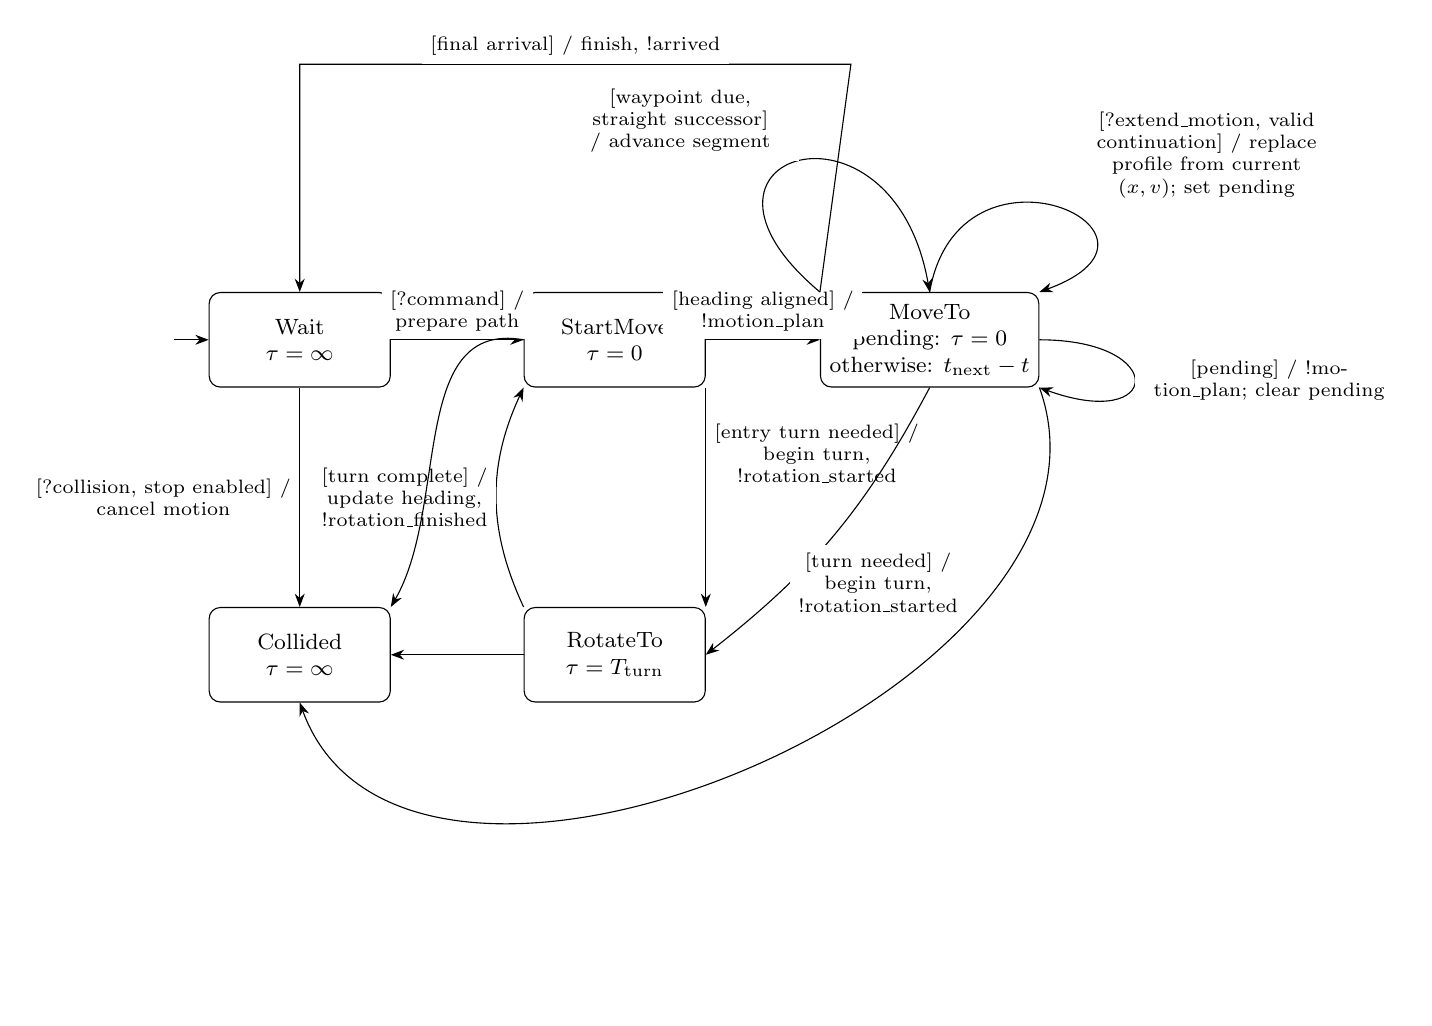
\begin{tikzpicture}[>=Stealth,every node/.style={font=\footnotesize},
 phase/.style={draw,rounded corners,align=center,minimum width=23mm,minimum height=12mm},
 lab/.style={align=center,fill=white,inner sep=3pt,font=\scriptsize}]
\node[phase] (w) at (0,0) {Wait\\$\tau=\infty$};
\node[phase] (s) at (4,0) {StartMove\\$\tau=0$};
\node[phase] (m) at (8,0) {MoveTo\\pending: $\tau=0$\\otherwise: $t_{\rm next}-t$};
\node[phase] (r) at (4,-4) {RotateTo\\$\tau=T_{\rm turn}$};
\node[phase] (c) at (0,-4) {Collided\\$\tau=\infty$};
\draw[->] (-1.6,0)--(w);
\draw[->] (w)--node[lab,above]{[?command] /\\prepare path}(s);
\draw[->] (s)--node[lab,above]{[heading aligned] /\\!motion\_plan}(m);
\draw[->] (s.south east) -- node[lab,right,pos=.3]{[entry turn needed] /\\begin turn,\\!rotation\_started}(r.north east);
\draw[->] (m.south) to[bend left=12] node[lab,right,pos=.7]{[turn needed] /\\begin turn,\\!rotation\_started}(r.east);
\draw[->] (r.north west) to[bend left=25] node[lab,left,pos=.5]{[turn complete] /\\update heading,\\!rotation\_finished}(s.south west);
\draw[->] (m.north west) -- (7,3.5) --node[lab,above]{[final arrival] / finish, !arrived}(0,3.5)--(w.north);
\draw[->] (m.north) to[out=80,in=20,looseness=4]
 node[lab,above right,text width=36mm]{[?extend\_motion, valid continuation] / replace profile from current $(x,v)$; set pending}(m.north east);
\draw[->] (m.east) to[out=0,in=-20,looseness=7]
 node[lab,right,text width=32mm]{[pending] / !motion\_plan; clear pending}(m.south east);
\draw[->] (m.north west) to[out=140,in=100,looseness=5]
 node[lab,above left,text width=28mm]{[waypoint due, straight successor] / advance segment}(m.north);
\draw[->] (w)--node[lab,left]{[?collision, stop enabled] /\\cancel motion}(c);
\draw[->] (s.west) to[out=170,in=60] (c.north east);
\draw[->] (m.south east) to[out=-70,in=-70] (c.south);
\draw[->] (r.west)--(c.east);
\end{tikzpicture}}
\caption{제어기 연장 명령을 포함한 MRobot 전이. 대기 중인 프로파일 출력은 동일 시각의 일반 경유점 전이보다 앞선다. 랙 처리의 LiftRack과 LowerRack은 생략했다. 모든 운전 상태에 Wait 엣지의 충돌 정지 조건과 취소 동작이 적용된다.}
\label{fig:mrobot-phases}
\end{figure}

\clearpage
\subsection{PSensor의 이벤트 기반 해제 센싱}
PSensor는 각 직선 이동의 프로파일, 시작 시각, 경로점, 방향 및 직사각형 반치수를 받는다. 이동 거리 $d_{\rm leave}$에서 몸체가 경로점을 완전히 비우면, 프로파일의 거리 역함수로 $t_0+T^{-1}_{\rm distance}(d_{\rm leave})$에 보고를 예약한다. 보고 값은 해제 시점의 로봇 중심이다. 주기적 위치 보고 대신 해제에 필요한 정보를 전송하며, 같은 시각 보고는 묶고 명령이 끝날 때까지 점유한 점은 해제로 보고하지 않는다.
\begin{figure}[htbp]
\centering
\resizebox{0.98\linewidth}{!}{%
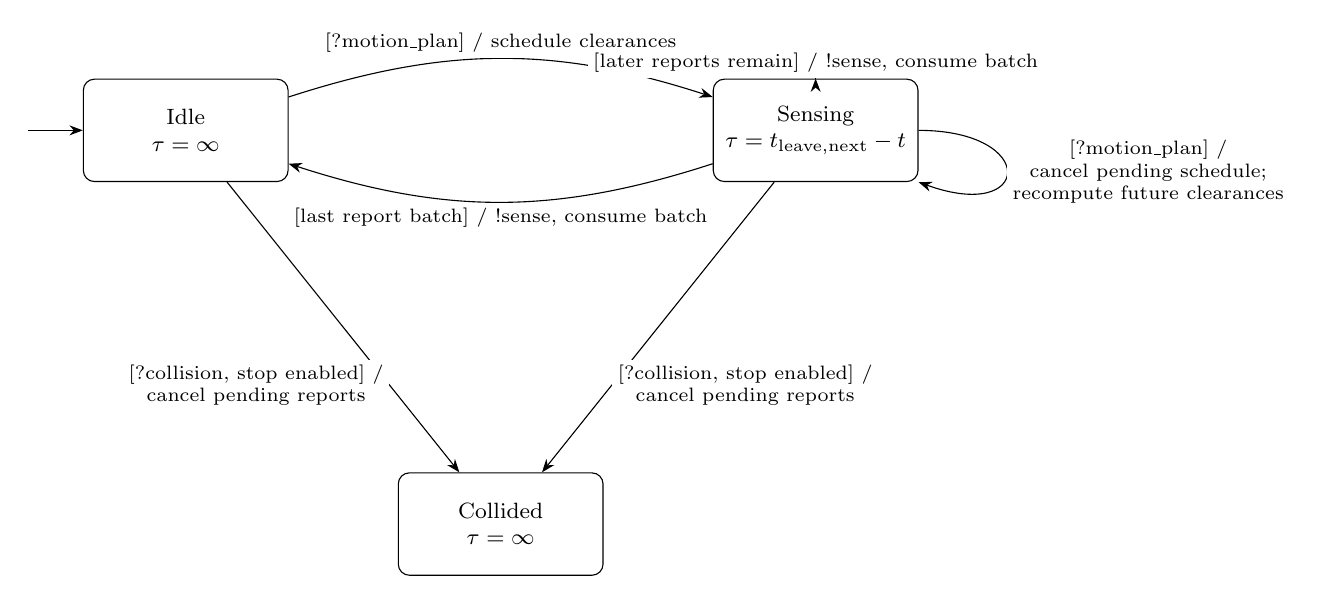
\begin{tikzpicture}[>=Stealth,every node/.style={font=\footnotesize},
 phase/.style={draw,rounded corners,align=center,minimum width=26mm,minimum height=13mm},
 lab/.style={align=center,fill=white,inner sep=2pt,font=\scriptsize}]
\node[phase] (i) at (0,0) {Idle\\$\tau=\infty$};
\node[phase] (s) at (8,0) {Sensing\\$\tau=t_{\rm leave,next}-t$};
\node[phase] (c) at (4,-5) {Collided\\$\tau=\infty$};
\draw[->] (-2,0)--(i);
\draw[->] (i) to[bend left=18] node[lab,above]{[?motion\_plan] / schedule clearances}(s);
\draw[->] (s) to[bend left=18] node[lab,below]{[last report batch] / !sense, consume batch}(i);
\draw[->] (s.north) to[out=60,in=120,looseness=10] node[lab,above]{[later reports remain] / !sense, consume batch}(s.north);
\draw[->] (s.east) to[out=0,in=-20,looseness=6] node[lab,right]{[?motion\_plan] /\\cancel pending schedule;\\recompute future clearances}(s.south east);
\draw[->] (i)--node[lab,left,pos=.7]{[?collision, stop enabled] /\\cancel pending reports}(c);
\draw[->] (s)--node[lab,right,pos=.7]{[?collision, stop enabled] /\\cancel pending reports}(c);
\end{tikzpicture}}
\caption{구현된 PSensor의 상태 전이. 예정 해제가 없으면 Sensing의 시간 전진은 무한대다.}
\label{fig:psensor-phases}
\end{figure}
충돌 정지를 끄면 PSensor는 충돌 입력을 무시하고 MRobot은 충돌 상태 표시와 함께 계속 움직인다. 검증은 충돌 정지를 사용한다. PSensor는 바로 Collided에 진입하며 별도의 충돌 보고 전이는 없다.

\clearpage
\subsection{예측 없이 실제 해제로 이동 목적지 연장}
이 선택적 실험 기능은 보고한 정차 기준에서는 꺼져 있다. 실제 Plant 해제로 다음 구간이 허용되면 제어기가 연장한다. TrafficManager는 FIFO와 필수 선행 검사를 유지하고 RoadMap에 새 부분을 예약한 뒤 RMFSController의 명령 버퍼에 넣는다. 이 부록의 해제 기반 구현은 예상 시간 차이로 진입을 허가하지 않으며, 삭제된 \texttt{!motion\_status} 요청·응답을 사용하지 않는다.
\begin{figure}[htbp]
\centering
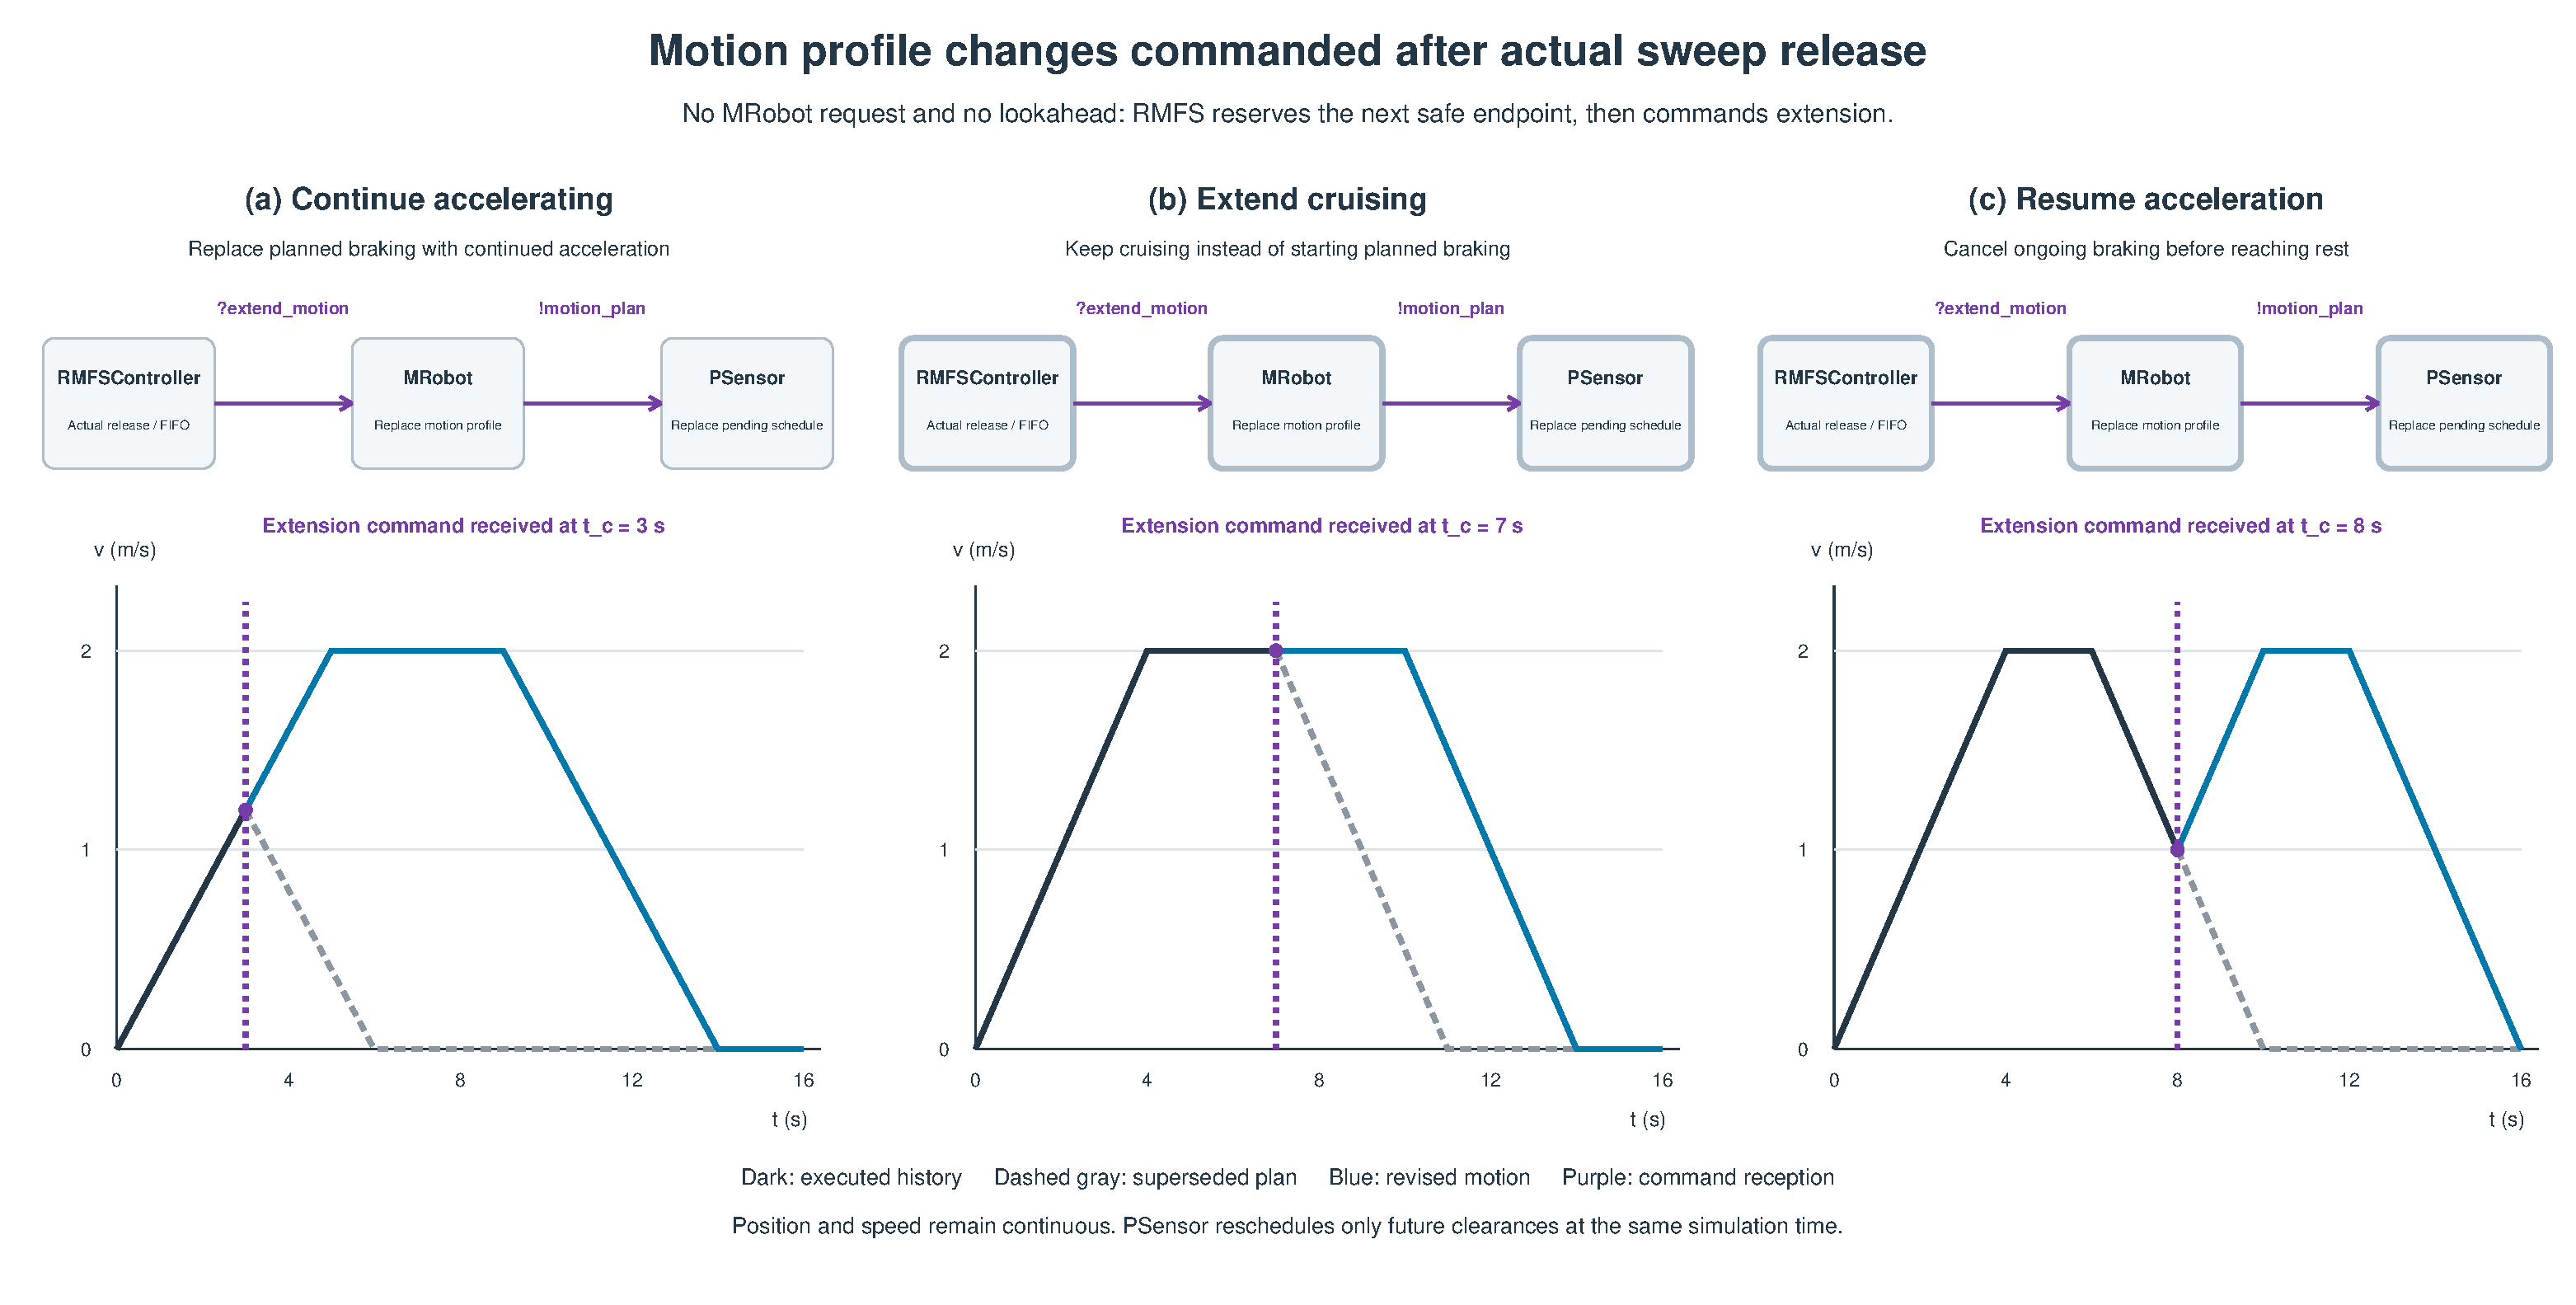
\includegraphics[width=\linewidth]{motion_profile_changes.pdf}
\caption{실제 스윕 해제 후 제어기가 지시한 운동 변경. 보라색 표지는 연장 명령 수신 시각이다. MRobot은 실행된 앞부분을 보존하고 이후 프로파일을 바꾸며, 0시간 출력으로 PSensor를 갱신한다. 가속 지속, 정속 연장, 감속 중 재가속을 설명한 도식이다.}
\label{fig:release-driven-profile}
\end{figure}

가속 중에는 계속 가속하고, 정속 중에는 감속을 늦추며, 감속 중에는 속도가 0에 이르기 전에 재가속할 수 있다. 연장은 같은 방향의 마지막 직선 구간에 적용한다. 회전은 기존 정차·회전을 사용한다. 이미 정차했으면 일반 이동 명령을 발행하며, 연장 허가가 없으면 원래 정차를 유지한다.

$t_c$는 명령 수신 시각, $u=v(t_c)$는 현재 속도, $D$는 새 종점까지의 직선 거리, $a,b>0$는 가감속 크기, $v_{\max}$는 속도 한계다. $D\ge u^2/(2b)$일 때 남은 프로파일은 다음과 같다.
\begin{equation}
 w=\min\!\left(v_{\max},
 \sqrt{\frac{2D+u^2/a}{1/a+1/b}}\right),\qquad
 t_a=\frac{w-u}{a},\qquad
 t_v=\frac{D-(w^2-u^2)/(2a)-w^2/(2b)}{w}.
 \label{eq:extension-tail}
\end{equation}
$w$는 새 최대속도, $t_a$는 가속시간, $t_v$는 정속시간(삼각형의 경우 0)이며 감속시간은 $w/b$다. $t_c$에서 위치와 속도는 연속이고 가속도는 바뀔 수 있다. \texttt{ExtendedProfile}은 이미 실행한 거리-시간 부분을 보존하고 $t_c$부터 새로운 나머지를 연결한다.

\paragraph{센서 일정 교체}
같은 시각 MRobot은 수정 프로파일, 원래 직선 시작 위치와 시각, 방향, 중간점 및 반치수를 보낸다. PSensor는 미보고 일정을 취소하고 새 역함수로 후속 해제를 계산한다. 지난 해제는 중복 보고하지 않는다. 중심이 이미 지났어도 몸체가 계속 덮고 있는 점은 앞으로 해제 보고를 할 수 있다. 종점에 도착해도 점유는 유지된다. 이 보고는 RoadMap을 갱신하고 선행 로봇이 움직이는 도중에도 FIFO 대기자를 재검토할 수 있게 한다. 스냅샷은 수정 프로파일과 0시간 출력 및 센서 일정을 보존해 남은 실행을 재현한다.

\paragraph{실행 가능한 점검 예제}
아래 3대 예제는 일반 DEVS 엔진, 실제 해제 보고, FIFO 및 분스합을 사용한다.
\begin{quote}\small\ttfamily
python -m examples.RMFS.Tests.03\_09\_RobotPath\_FIFO\_ReleaseExtension
\end{quote}
Space는 한 이벤트, A는 자동 재생, R은 초기화다. 빈 로봇 사례에서 R2는 8.000~s에 감속을 시작한다. R1이 9.878~s에 도착해 해제하면 R2가 아직 감속 중이므로 이동을 연장한다. R2는 양의 속도에서 재가속하며 PSensor가 일정을 교체한다. 0.1~s 간격 충돌 정지 검증에서 검출 접촉 없이 세 경로가 25.101~s에 완료됐다. 이 결과는 보고된 시뮬레이션 사례에 해당한다.

\end{document}
